% Supplementary material for "Benchmarking LLM Integration Strategies for
% MCDA-Assisted Household Energy Decision Support" (Environmental Modelling & Software).
% Compile separately from the main paper; the bibliography is shared (cas-refs.bib).
\documentclass[11pt]{article}
\usepackage[margin=1in]{geometry}
\usepackage{amsmath,amssymb}
\usepackage{booktabs}
\usepackage{multirow}
\usepackage{threeparttable}
\usepackage{alltt}
\usepackage{float}
\usepackage{textcomp}
\usepackage{xcolor}
\definecolor{colorPure}{RGB}{180,180,180}
\definecolor{colorRAG}{RGB}{100,149,200}
\definecolor{colorLLMParameterizedReferenceScoring}{RGB}{31,73,125}
\definecolor{colorGemini}{HTML}{E69F00}
\definecolor{colorDeepSeek}{HTML}{56B4E9}
\definecolor{colorGPTOSS}{HTML}{009E73}
\definecolor{colorQwen}{HTML}{D55E00}
\usepackage{listings}
\definecolor{jsonbg}{RGB}{247,247,247}
\definecolor{jsonframe}{RGB}{200,200,200}
\definecolor{jsonstring}{RGB}{20,120,20}
\lstdefinestyle{jsonstyle}{
  basicstyle=\ttfamily\footnotesize,
  backgroundcolor=\color{jsonbg},
  frame=single,
  rulecolor=\color{jsonframe},
  framesep=4pt,
  breaklines=true,
  showstringspaces=false,
  columns=fullflexible,
  keepspaces=true,
  moredelim=[s][\color{jsonstring}]{"}{"},
  xleftmargin=4pt,
  xrightmargin=4pt,
}
\usepackage{tikz}
\usepackage{pgfplots}
\pgfplotsset{compat=1.18}
\usepackage[hidelinks]{hyperref}
\usepackage[authoryear,longnamesfirst]{natbib}

\newcounter{suppsectioncounter}
\newcommand{\suppsection}[1]{%
  \stepcounter{suppsectioncounter}%
  \section*{S\thesuppsectioncounter.\ #1}%
  \setcounter{table}{0}\setcounter{figure}{0}\setcounter{equation}{0}%
  \renewcommand{\theHtable}{S\thesuppsectioncounter.\arabic{table}}%
  \renewcommand{\theHfigure}{S\thesuppsectioncounter.\arabic{figure}}%
}
\renewcommand{\thetable}{S\thesuppsectioncounter.\arabic{table}}
\renewcommand{\thefigure}{S\thesuppsectioncounter.\arabic{figure}}
\renewcommand{\theequation}{S\thesuppsectioncounter.\arabic{equation}}

\title{Supplementary Material: Benchmarking LLM Integration Strategies for MCDA-Assisted Household Energy Decision Support}
\author{Ahaan Nigam and River Huang}
\date{}
\begin{document}
\maketitle
\suppsection{Extended Methods}
\label{app:model_routing}

The four models and their exact OpenRouter identifiers are GPT-OSS-20B (\texttt{openai/gpt-oss-20b:exacto}, reasoning, low effort), Qwen 3.5 9B (\texttt{qwen/qwen3.5-9b:exacto}, non-reasoning), DeepSeek V4 Flash (\texttt{deepseek/deepseek-v4-flash:exacto}, hybrid reasoning), and Gemini 3.5 Flash 

\noindent(\texttt{google/gemini-3.5-flash:exacto}, reasoning, minimal effort). The \texttt{:exacto} suffix is an OpenRouter provider-routing variant that restricts serving to providers meeting a fixed accuracy standard; it is part of the model identifier and is required to reproduce these runs.

At least two alternatives share a weighted score in 3.2\% of Gemini's $\mathcal{A}_{\text{D}}$ scenarios, 5.9\% of DeepSeek's, 12.6\% of GPT-OSS's and 21.3\% of Qwen's, and in 2.7\%, 19.1\%, 6.4\% and 13.9\% of the same four models' $\mathcal{A}_{\text{E}}$ scenarios. All three alternatives carrying identical scores on all four criteria is rarer, between 0.0\% and 1.2\% in every model--architecture cell, so the tie-break rule usually separates alternatives that already differ on at least one criterion.
\subsection{Full Prompt Texts}
\label{app:prompts}

Full verbatim text of the system and extraction prompts, in the order the architectures appear in the framework.

\subsection{\texorpdfstring{$\mathcal{A}_{\text{D}}$}{A\_D} System Prompt}

\begin{minipage}{\columnwidth}
\begin{alltt}
\footnotesize
\textbf{System prompt:}

You are an expert household decision analyst specializing in Multi-Criteria Decision
  Analysis (MCDA).
You consistently utilize all information given in the scenario context. Score alternatives
  on four criteria using the inclusive 0-1 scale (0.0 <= score <= 1.0):

HVAC:
- energy\_cost: good when the setpoint demands little from the system given outdoor
  conditions; moderate when the system must work harder; poor when the setpoint requires
  extreme effort.
- environmental: good when the system runs efficiently; moderate when runtime and load are
  average; poor when high load drives sustained high emissions.
- comfort: good when the setpoint feels comfortable for the outdoor temperature; moderate
  when slightly outside typical preference; poor when noticeably too hot or cold.
- practicality: good when the setpoint is easy for the user and system to maintain without
  strain; moderate when borderline; poor when extreme enough to risk override or system
  stress.

Appliance (scheduling):
- energy\_cost: good during off-peak rate hours; moderate in shoulder periods; poor when
  scheduled during peak pricing windows.
- environmental: good when grid emissions are low (typically overnight); moderate during
  shoulder hours; poor when peak-period generation is dirtiest.
- comfort: good when the appliance is available with little or no delay; moderate when
  availability is pushed later into the evening; poor when results are not ready until the
  following morning.
- practicality: good when scheduling is easy to remember and socially unobtrusive;
  moderate when timing requires some planning; poor when running in the middle of the
  night creates noise or coordination difficulty.

Shower (duration):
- energy\_cost: good when short; worsens continuously as duration increases.
- environmental: good when water volume used is low; worsens continuously as duration
  increases.
- comfort: good near a typical shower length; poor when too short to feel adequate or long
  enough to feel wasteful.
- practicality: good when the duration is sustainable as a daily habit; poor when too
  short to realistically maintain or long enough to cause hot water contention.
\end{alltt}
\end{minipage}

\smallskip
\noindent\textbf{Output format (return ONLY this JSON):}
\begin{lstlisting}[style=jsonstyle]
{
  "energy_cost": X,
  "environmental": X,
  "comfort": X,
  "practicality": X
}
\end{lstlisting}
\noindent where each X is between 0.0 and 1.0. You must distinguish between the criteria: do not assign the same score to all 4 criteria for an alternative unless performance is actually identical across them.

\noindent The user prompt includes the other alternatives as reference so that it doesn't assign the same scores to all alternatives.

\subsection{\texorpdfstring{$\mathcal{A}_{\text{E}}$}{A\_E} System Prompt}

\begin{minipage}{\columnwidth}
\begin{alltt}
\footnotesize
\textbf{System prompt:}

You are an expert household decision analyst specializing in Multi-Criteria Decision
  Analysis (MCDA).
You consistently utilize all information given in the scenario context. Score alternatives
  on four criteria using the inclusive 0-1 scale (0.0 <= score <= 1.0):
1. Energy Cost: Lower energy costs = higher score.
2. Environmental Impact: Lower emissions = higher score.
3. Comfort: Higher user comfort = higher score.
4. Practicality: Easier to implement/maintain = higher score.
\end{alltt}
\end{minipage}

\smallskip
\noindent\textbf{Output format (return ONLY this JSON):}
\begin{lstlisting}[style=jsonstyle]
{
  "energy_cost": X,
  "environmental": X,
  "comfort": X,
  "practicality": X
}
\end{lstlisting}
\noindent where each X is between 0.0 and 1.0. You must distinguish between the criteria: do not assign the same score to all 4 criteria for an alternative unless performance is actually identical across them.

\subsection{\texorpdfstring{$\mathcal{A}_{\text{H}}$}{A\_H} Extraction Prompt}

\begin{minipage}{\columnwidth}
\begin{alltt}
\footnotesize
\textbf{Extraction prompt:}

You are a household-systems engineer. You base all assumptions off of given information.
  Understand how each parameter affects another. When extrapolating missing values, use
  all information given to specify a reasonable value for the value being extrapolated.

SCENARIO:
\{scenario\_text\}

QUESTION: \{question\}

INSTRUCTIONS:
1. Identify the Decision Type: HVAC, Appliance, or Shower.
2. Estimate ONLY the parameters listed for that type below.
3. Every listed parameter is mandatory. If a value is not stated, it is mandatory to
  reasonably estimate it from the scenario context.
4. Return ONLY valid JSON in the exact structure shown.
\end{alltt}
\end{minipage}

\smallskip
\noindent\textbf{For HVAC decisions:}
\begin{lstlisting}[style=jsonstyle]
{
  "decision_type": "HVAC",
  "calculator": "HVACGroundTruthCalculator",
  "parameters": {
    "r_value": <number>,
    "seer": <number>,
    "hvac_age": <number>,
    "occupancy_context": "occupied_all_day | unoccupied_<hours> | occupied_sleep"
  }
}
\end{lstlisting}

\noindent\textbf{For Appliance decisions:}
\begin{lstlisting}[style=jsonstyle]
{
  "decision_type": "Appliance",
  "calculator": "ApplianceGroundTruthCalculator",
  "parameters": {
    "appliance": "Dishwasher | Washer | Dryer",
    "kwh_per_cycle": <number>,
    "baseline_time": "<the time it currently is, e.g. 7pm, 8am>"
  }
}
\end{lstlisting}

\noindent\textbf{For Shower decisions:}
\begin{lstlisting}[style=jsonstyle]
{
  "decision_type": "Shower",
  "calculator": "ShowerGroundTruthCalculator",
  "parameters": {
    "gpm": <number>,
    "tank_size": <number>,
    "water_heater_temp": <number>
  }
}
\end{lstlisting}

\noindent Return ONLY the JSON, no explanation.

\subsection{Retrieved Exemplar Rendering}
\noindent A retrieved HVAC exemplar (engineering parameters and ground-truth scores included) is rendered as:

\begin{alltt}
\footnotesize
RELEVANT SIMILAR SCENARIOS WITH EXPERT SCORES:

Example 1:
  Question: I'm heading out for a quick errand, what AC temperature should I set for the
    townhouse?
  - Location: King of Prussia, PA
  - Outdoor Temp: 93 deg F
  - Square Footage: 2200 sqft
  - Insulation: Medium
  - Household Size: 5 occupants
  - Housing Type: Townhouse
  - House Age: 11-15 years
  - R-Value: 17
  - SEER: 15
  - HVAC Age: 12 years
  - Utility Budget: \$285/month
  Expert scores:
  * 75 F: Energy Cost: 0.5/1, Environmental: 0.5/1,
    Comfort: 0.9/1, Practicality: 0.8/1
    | MAVT: 0.61, Rank: 2
  * 78 F: Energy Cost: 0.5/1, Environmental: 0.5/1,
    Comfort: 0.8/1, Practicality: 0.8/1
    | MAVT: 0.62, Rank: 1
  * 81 F: Energy Cost: 0.5/1, Environmental: 0.5/1,
    Comfort: 0.5/1, Practicality: 0.8/1
    | MAVT: 0.58, Rank: 3
Use these examples as reference, but score based on
the specific scenario above.
\end{alltt}\subsection{RAG Corpus Description}
\label{app:rag_corpus}

The retrieval-augmented generation (RAG) corpus consists of 90 unique
scenarios (35 HVAC, 35 Appliance, 20 Shower) that are disjoint
from the 195 test scenarios. Each RAG scenario has three alternatives,
yielding 270 total rows across the three source files
(HVACRagScenarios.xlsx, ApplianceRAGScenarios.xlsx,
ShowerRAGScenarios.xlsx).

Scenarios were generated from the same parameter distribution as the test
set but kept separate to prevent any test scenario from appearing in the
retrieval index. A combinatorial audit ensured that no parameter
combination was underrepresented: each categorical cross-cell (insulation
tier $\times$ housing type, appliance type $\times$ flow-rate band, etc.)
contained at least one scenario, and the 90 RAG scenarios were drawn from
this audited matrix. The 195 test scenarios were built and rebalanced
against the same audited matrix, so that every categorical combination
appears at least once in each decision type's test set.

The retrieval index was built using the
\texttt{sentence-transformers/all-MiniLM-L6-v2} embedding model
\citep{reimers2019sentencebert}, producing 384-dimensional dense vectors.
At query time, the single most similar scenario ($k=1$) is retrieved by
Euclidean (L2) distance, Chroma's default metric, and rendered as a full worked example in the LLM prompt.
The embedding string includes all household-reported parameters (location,
square footage, insulation tier, household size, housing type, utility
budget, outdoor temperature, house age) plus band labels for age and flow
rate, but excludes engineering parameters and ground-truth scores, which
appear only in the display metadata of the retrieved exemplars.

The disjointness of test and RAG sets was verified by construction (the
rebuild script exports them from separate master-sheet partitions).

\subsection{Parameter Ranges and Band Labels}
\label{app:parameter_ranges}

Each insulation tier spans a range of R-values drawn from standard U.S.\ residential wall assemblies \citep{cec_ja43_2013,energystar_insulation2023}: Poor scenarios use R-8 to R-12 (minimal 2$\times$4 cavity fill, below current code), Medium scenarios use R-13 to R-18 (standard 2$\times$4 batt through 2$\times$6 mixed), and Good scenarios use R-19 to R-24 (2$\times$6 framing and above). Consecutive tier midpoints differ by 55\% (R-10 to R-15.5) and 39\% (R-15.5 to R-21.5) in wall R-value. SEER ratings in the test corpus span 8--22, covering pre-1992 units (SEER~8--10), standard-efficiency replacements (SEER~13--14), and high-efficiency models (SEER~16--22), consistent with the ENERGY STAR Most Efficient threshold \citep{energystar_ac2023}.

The appliance age presented to the LLM architectures is a band label (1--3, 4--6, 7--9, 10--12, 13--17, and 28--32 years in the test corpus), derived from the scenario's raw integer age by a single shared helper so that the label is byte-identical on the query and index sides of retrieval. The scenario sheets retain both the raw age and an independent per-cycle energy value (kWh/cycle) drawn from the ENERGY STAR certified-products database, and the ground-truth calculator scores kWh/cycle directly without reference to age. Within a single appliance type the band and the per-cycle energy are only moderately associated (Spearman's $\rho = 0.36$ for dishwashers, $0.38$ for dryers, and $0.69$ for washing machines), so two appliances sharing a band can differ materially in energy draw---a 7--9~year dryer ranges from 2.40 to 3.50\,kWh/cycle across the corpus.

For the Flow Rate parameter, the scenario's numeric GPM is bucketed into three qualitative labels: \texttt{low\_flow} ($\le$2.0\,GPM, including EPA WaterSense certified showerheads \citep{epawatersense}), \texttt{standard} (2.5--3.0\,GPM, at or near the Energy Policy Act of 1992 federal maximum of 2.5\,GPM \citep{epawatersense}), and \texttt{high\_flow} ($>$3.0\,GPM). The label is present in the LLM test scenarios only, and is mapped from those ranges to the actual numeric GPM from the actual scenario.
\subsection{Worked Example: \texorpdfstring{$\mathcal{A}_{\text{H}}$}{A_H} HVAC Scenario}
\label{app:hvac_worked}

This subsection traces one HVAC scenario end-to-end through the
$\mathcal{A}_{\text{H}}$ pipeline. The full step-by-step arithmetic
(thermal load, EER conversion, energy/cost/emissions, budget penalty,
comfort and practicality scores, value-function transformation) is
reproducible by running \texttt{Ground Truth Calculators/HVACGroundTruthCalculator.py}
in the project repository on the scenario below; only the inputs and the
final result are shown here.

The scenario: Philadelphia, PA; outdoor temperature $95\,^\circ\text{F}$
(cooling season); 2{,}200\,sq\,ft single-family home, medium insulation,
house age 15\,years; household size 4; \$200/month utility budget;
alternatives of $72\,^\circ\text{F}$, $76\,^\circ\text{F}$, and
$80\,^\circ\text{F}$. $\mathcal{A}_{\text{H}}$'s extraction step returns
$R=15$, $\text{SEER}=13$, $\text{hvac\_age}=10$, and
\texttt{occupancy\_context}\,=\,\texttt{occupied\_all\_day}, each validated
against the physically admissible bounds
before being merged with the household-reported fields above and the fixed
electricity rate of \$0.19/kWh to produce the full scenario dict passed to
\texttt{HVACGroundTruthCalculator}.

Carrying that scenario through the HVAC calculator equations above
for all three alternatives yields:
\begin{center}
\begin{tabular}{@{}lrrrrr@{}}
\toprule
\textbf{Setpoint} & \textbf{$v_{\text{cost}}^{*}$} & \textbf{$v_{\text{env}}$}
  & \textbf{$v_{\text{comfort}}$} & \textbf{$v_{\text{prac}}$}
  & \textbf{MAVT $s_j$} \\
\midrule
$76\,^\circ$F & 0.11 & 0.30 & 1.00 & 0.85 & \textbf{0.466} \\
$80\,^\circ$F & 0.17 & 0.37 & 0.67 & 0.85 & 0.441 \\
$72\,^\circ$F & 0.06 & 0.24 & 0.67 & 0.78 & 0.352 \\
\bottomrule
\end{tabular}
\end{center}
\subsection{GPT-OSS Extraction Failure Analysis}
\label{app:extraction_failure_analysis}
The $\mathcal{A}_{\text{H}}$ architecture validates each extracted JSON
before passing it to the ground-truth calculator. A scenario is recorded
as an extraction failure when: the LLM response is not valid JSON; a
required parameter is absent; a numeric parameter parses as non-finite or
falls outside its physically admissible range; or the extracted decision
type does not match the scenario's known type.

GPT-OSS 20B exhibited a 33.4\% extraction failure rate on
$\mathcal{A}_{\text{H}}$ HVAC scenarios (12.0\% across all decision types),
triggered entirely by invalid parameters. All of its $\mathcal{A}_{\text{H}}$
failures were HVAC scenarios; Appliance and Shower extraction succeeded in
every run. In a typical failure the model returns well-formed JSON but
estimates parameters outside the validation bounds---for example, a SEER rating of 5 against a
lower bound of 6.0. The validation layer detects the out-of-range value,
flags the scenario as an extraction failure, and assigns the sentinel
value (1928) to all four criterion scores for that scenario.

Table~\ref{tab:failure_modes} breaks the failure counts down by failure mode. The most common failure mode for $\mathcal{A}_{\text{D}}$ and $\mathcal{A}_{\text{E}}$ is \texttt{EXTRACTION\_INVALID\_\allowbreak JSON} (model returns unparseable output), while for $\mathcal{A}_{\text{H}}$, all failures concentrate in \texttt{FAILED\_EXTRACTION\_\allowbreak INVALID\_\allowbreak PARAMETERS} (extracted numeric parameter falls outside the physical validation bounds), driven almost entirely by GPT-OSS on HVAC scenarios.

\begin{table}[htbp]
\small\centering
\caption{Nonzero-firing failure mode counts per architecture (5-run total across all models).\protect\footnotemark}
\label{tab:failure_modes}
\begin{tabular}{lccc}
\toprule
Mode & $\mathcal{A}_{\text{D}}$ & $\mathcal{A}_{\text{E}}$ & $\mathcal{A}_{\text{H}}$ \\
\midrule
\texttt{EXTRACTION\_INVALID\_JSON} & 5 & 11 & 0 \\
\texttt{FAILED\_MISSING\_SCORE} & 1 & 0 & 0 \\
\texttt{FAILED\_EXTRACTION\_INVALID\_PARAMETERS} & 0 & 0 & 120 \\
\bottomrule
\end{tabular}
\footnotetext{Counts are 5-run totals summed across all four models, on a mode-occurrence basis (one count per failure code firing on a given run). Of fifteen possible failure codes, only these three ever fired across all 60 runs; the remaining twelve were checked and never triggered. These totals (6/11/120) differ from unique-scenario-run totals (9/10/120) because a unique failed scenario-run does not always map to exactly one mode-occurrence: for $\mathcal{A}_{\text{D}}$, three scenario-run failures have no single attributable mode code recorded; for $\mathcal{A}_{\text{E}}$, one scenario-run failure triggered its mode code twice across its alternative-scoring calls.}
\end{table}
\subsection{Pennsylvania Time-of-Use Rate Structure}
\label{app:tou_rates}

Table~\ref{tab:tou_rates} lists the six Pennsylvania utilities used by
the appliance ground-truth calculator, with their TOU peak/off-peak
windows and energy rates (\$/kWh). All scenarios use weekday summer rates
year-round; seasonal peak-window shifts (e.g., PPL winter 4--8pm vs.\
summer 2--6pm) and weekend off-peak pricing are not modeled.

\begin{table}[t]
\small
\centering
\renewcommand{\arraystretch}{1.15}
\caption{Pennsylvania utility TOU rate structure. Peak window is
24-hour clock (start, end). All rates in \$/kWh. The residential
electricity rate of \$0.19/kWh used for HVAC cost normalization is the
statewide bundled baseline \citep{eia_epa_2024,paupc2025}.}
\label{tab:tou_rates}
\begin{tabular}{@{}l cc rr@{}}
\toprule
\textbf{Utility} & \textbf{Peak Window} & \textbf{Peak Rate} &
  \textbf{Off-Peak Rate} \\
\midrule
PECO       & 2--6pm  & 0.3200 & 0.0760 \\
PPL        & 2--6pm  & 0.1600 & 0.0700 \\
West Penn  & 2--9pm  & 0.1720 & 0.0880 \\
Penelec    & 2--9pm  & 0.1850 & 0.0930 \\
MetEd      & 2--9pm  & 0.2030 & 0.1000 \\
Duquesne   & 2--9pm  & 0.1375 & 0.1375 \\
\bottomrule
\end{tabular}
\renewcommand{\arraystretch}{1.0}
\end{table}

PECO (Rate R-TOU) \citep{peco2021} and PPL (Rate RTS) \citep{ppl2025} use a 4-hour afternoon peak window (2--6pm weekdays). The three FirstEnergy utilities (West Penn, Penelec, MetEd) use a 7-hour peak window (2--9pm weekdays), with rates derived from the Jun-2025 Price-to-Compare (PTC) multiplied by approved multipliers \citep{firstenergy2025,firstenergy2026}. Duquesne uses a flat default rate (Rate RS) \citep{duquesne2026}. Shifting a dishwasher cycle from peak to off-peak cuts its per-cycle cost by 49--76\% across these five time-of-use utilities.
\subsection{Realized Criterion Swing}
\label{app:swing_weights}

Table~\ref{tab:swing_weights} reports, for each criterion and decision type, the mean over scenarios of the nominal weight times the within-scenario score range---the quantity each criterion actually contributes to the spread in MAVT score within a choice set, as distinct from its nominal weight.

\begin{table*}[htbp]
\centering
\begin{threeparttable}
\footnotesize
\centering
\renewcommand{\arraystretch}{1.15}
\begin{tabular}{lcccc}
\toprule
Criterion & Nominal Weight & HVAC & Appliance & Shower \\
\midrule
Energy Cost & 0.30 & 0.027 & 0.066 & 0.108 \\
Environmental Impact & 0.35 & 0.032 & 0.008 & 0.128 \\
Comfort & 0.20 & 0.086 & 0.098 & 0.070 \\
Practicality & 0.15 & 0.015 & 0.095 & 0.053 \\
\bottomrule
\end{tabular}
\renewcommand{\arraystretch}{1.0}
\end{threeparttable}
\caption{Mean within-scenario swing (nominal weight $\times$ within-scenario score range) by criterion and decision type.}
\label{tab:swing_weights}
\end{table*}

\subsection{Full Sensitivity Analysis Results}
\label{app:sensitivity_full}

Table~\ref{tab:sensitivity_by_model} gives Kendall's~$\tau$ for every model,
architecture and weight vector. Table~\ref{tab:sensitivity_top1} gives Top-1
accuracy for the same cells. The weight vectors are the design vector
$(0.30,\,0.35,\,0.20,\,0.15)$, the equal-weight vector
$(0.25,\,0.25,\,0.25,\,0.25)$, and the entropy- and MEREC-derived vectors of
Appendix~B, each applied pooled across the corpus and per decision type. No
value in either table is pooled across models.

\begin{table*}[htbp]
\centering
\begin{threeparttable}
\footnotesize
\centering
\textbf{Sensitivity analysis: Kendall's $\tau$ by model under reweighting}
\renewcommand{\arraystretch}{1.15}
\setlength{\tabcolsep}{4pt}
\begin{tabular}{@{} l rrr rrr rrr rrr @{}}
\toprule
 & \multicolumn{3}{c}{Gemini} & \multicolumn{3}{c}{DeepSeek} & \multicolumn{3}{c}{GPT-OSS} & \multicolumn{3}{c}{Qwen} \\
\cmidrule(lr){2-4}\cmidrule(lr){5-7}\cmidrule(lr){8-10}\cmidrule(lr){11-13}
\textbf{Weight vector} & $\mathcal{A}_{\text{D}}$ & $\mathcal{A}_{\text{E}}$ & $\mathcal{A}_{\text{H}}$ & $\mathcal{A}_{\text{D}}$ & $\mathcal{A}_{\text{E}}$ & $\mathcal{A}_{\text{H}}$ & $\mathcal{A}_{\text{D}}$ & $\mathcal{A}_{\text{E}}$ & $\mathcal{A}_{\text{H}}$ & $\mathcal{A}_{\text{D}}$ & $\mathcal{A}_{\text{E}}$ & $\mathcal{A}_{\text{H}}$ \\
\midrule
Design (baseline)  & 0.176 & 0.310 & 0.923 & 0.144 & 0.307 & 0.897 & 0.041 & 0.272 & 0.897 & 0.010 & 0.208 & 0.880 \\
Equal              & 0.312 & 0.389 & 0.911 & 0.115 & 0.311 & 0.909 & 0.081 & 0.267 & 0.877 & $-$0.028 & 0.225 & 0.879 \\
\midrule
Entropy pooled     & 0.197 & 0.331 & 0.919 & 0.126 & 0.314 & 0.873 & 0.039 & 0.279 & 0.880 & 0.004 & 0.197 & 0.848 \\
Entropy per-type   & 0.170 & 0.336 & 0.917 & 0.088 & 0.347 & 0.896 & 0.043 & 0.280 & 0.885 & $-$0.007 & 0.218 & 0.886 \\
\midrule
MEREC pooled       & \textbf{0.655} & 0.632 & 0.956 & 0.220 & 0.410 & 0.963 & 0.233 & 0.329 & 0.953 & 0.000 & 0.267 & 0.963 \\
MEREC per-type     & 0.602 & 0.625 & 0.929 & 0.308 & 0.367 & 0.930 & 0.163 & 0.372 & 0.900 & 0.041 & 0.248 & 0.921 \\
MEREC HVAC vector  & \textbf{0.676} & 0.600 & 0.985 & 0.333 & 0.413 & 0.984 & 0.275 & 0.427 & 0.976 & 0.064 & 0.282 & 0.984 \\
\bottomrule
\end{tabular}
\renewcommand{\arraystretch}{1.0}
\setlength{\tabcolsep}{6pt}
\begin{tablenotes}
\footnotesize
\item Both the reference ranking and the architecture ranking are recomputed under each vector, because a MAVT reference is defined by its weights. Bold marks the two cells in which $\mathcal{A}_{\text{D}}$ exceeds $\mathcal{A}_{\text{E}}$; both occur for Gemini under MEREC vectors. Top-1 accuracy for the same cells appears in Table~\ref{tab:sensitivity_top1} below.
\end{tablenotes}
\end{threeparttable}
\caption{Kendall's $\tau$ by model and architecture under seven weight vectors. No value is pooled across models.}
\label{tab:sensitivity_by_model}
\end{table*}

\begin{table*}[t]
\centering
\begin{threeparttable}
\footnotesize
\centering
\renewcommand{\arraystretch}{1.10}
\setlength{\tabcolsep}{4pt}
\caption{Sensitivity analysis: Top-1 accuracy (\%) by model and architecture under seven weight vectors.}
\label{tab:sensitivity_top1}
\begin{tabular}{@{}l rrr rrr rrr rrr@{}}
\toprule
 & \multicolumn{3}{c}{Gemini} & \multicolumn{3}{c}{DeepSeek} & \multicolumn{3}{c}{GPT-OSS} & \multicolumn{3}{c}{Qwen} \\
\cmidrule(lr){2-4}\cmidrule(lr){5-7}\cmidrule(lr){8-10}\cmidrule(lr){11-13}
\textbf{Weight vector} & $\mathcal{A}_{\text{D}}$ & $\mathcal{A}_{\text{E}}$ & $\mathcal{A}_{\text{H}}$ & $\mathcal{A}_{\text{D}}$ & $\mathcal{A}_{\text{E}}$ & $\mathcal{A}_{\text{H}}$ & $\mathcal{A}_{\text{D}}$ & $\mathcal{A}_{\text{E}}$ & $\mathcal{A}_{\text{H}}$ & $\mathcal{A}_{\text{D}}$ & $\mathcal{A}_{\text{E}}$ & $\mathcal{A}_{\text{H}}$ \\
\midrule
Design (baseline)  & 36.2 & 48.7 & 93.1 & 36.7 & 53.5 & 90.8 & 33.3 & 47.4 & 91.7 & 30.0 & 46.6 & 89.7 \\
Equal              & 50.0 & 55.0 & 94.4 & 36.8 & 52.5 & 93.7 & 37.7 & 48.5 & 92.7 & 28.8 & 46.2 & 89.5 \\
\midrule
Entropy pooled     & 37.5 & 48.9 & 93.7 & 35.5 & 54.2 & 89.8 & 33.7 & 48.5 & 91.7 & 29.6 & 46.5 & 88.4 \\
Entropy per-type   & 39.0 & 52.1 & 94.6 & 34.2 & 56.0 & 92.4 & 34.7 & 49.3 & 92.4 & 30.1 & 46.1 & 92.7 \\
\midrule
MEREC pooled       & \textbf{75.7} & 74.4 & 95.3 & 43.6 & 57.4 & 95.5 & 46.9 & 53.9 & 94.1 & 32.3 & 49.8 & 97.5 \\
MEREC per-type     & 69.1 & 76.1 & 93.8 & 49.4 & 52.6 & 94.5 & 41.5 & 57.0 & 92.3 & 34.5 & 50.0 & 92.2 \\
MEREC HVAC vector  & \textbf{80.4} & 71.5 & 98.5 & 53.6 & 56.5 & 97.9 & 49.1 & 61.1 & 96.9 & 37.1 & 51.6 & 99.2 \\
\bottomrule
\end{tabular}
\renewcommand{\arraystretch}{1.0}
\setlength{\tabcolsep}{6pt}
\begin{tablenotes}
\footnotesize
\item Percentage of the 195 test scenarios whose top-ranked alternative matches
the reference. Bold marks cells in which $\mathcal{A}_{\text{D}}$ exceeds
$\mathcal{A}_{\text{E}}$; these are the same two Gemini MEREC cells that reverse
on Kendall's~$\tau$.
\end{tablenotes}
\end{threeparttable}
\end{table*}

\subsection{Ablation Data Provenance}
\label{app:ablation_provenance}

The RAG and prompt-sensitivity ablations reported in this section were collected against an earlier shower comfort function. That function scored the water-heater setpoint, a storage temperature, against a 110--130\,\textdegree{}F no-penalty band taken from delivery-side comfort and scald thresholds. The shipped function uses 120--140\,\textdegree{}F, anchored instead to CDC storage guidance: below 120\,\textdegree{}F a tank cannot deliver the 105\,\textdegree{}F target with mixing margin and sits inside the \textit{Legionella} amplification range, and above 140\,\textdegree{}F adds standby loss without comfort benefit. The main manuscript's Calculator Simplifications subsection discusses the correction.

We recomputed the shower reference under the corrected band before deciding whether to re-collect. The setpoint enters comfort as a per-scenario constant shared by all three alternatives, so it moves a ranking only through the criterion balance. Across the 60 test shower scenarios the correction changes the reference winner in none and the full reference ranking in none. In the 20-scenario shower RAG corpus it changes 1 winner and 2 rankings. Both ablation suites test whether a configuration preserves the architecture ordering, and the narrowest ordering margin either suite resolves is 0.13 in Kendall's $\tau$, so a correction that moves no test reference winner cannot reverse either suite's conclusions. Additionally, 799 of 14,400 $\mathcal{A}_{\text{H}}$ Shower comfort cells (5.5\%) failed to reproduce under the uncorrected calculator because shipped scores omitted cold-weather duration elasticity. Realigning elasticity and applying the 120--140\,\textdegree{}F band yields $\tau = 0.8117$ versus shipped $0.8111$, confirming the gap is rank-neutral and affects score errors only. The headline results in the main text use the corrected reference throughout.

\subsection{RAG Ablation: Full Per-Configuration Table}
\label{app:rag_ablation_full}

\begin{table}[t]
\centering
\begin{threeparttable}
\small
\centering
\renewcommand{\arraystretch}{1.15}
\begin{tabular}{lcccc}
\toprule
Configuration & DeepSeek & Gemini & GPT-OSS & Qwen \\
\midrule
\multicolumn{5}{l}{\emph{Kendall's $\tau$}} \\
Exemplars w/o hidden params & 0.391 & 0.437 & 0.175 & 0.273 \\
$k{=}3$ control setting (all-MiniLM-L6-v2) & 0.489 & 0.387 & 0.187 & 0.154 \\
Alt.\ embedding & 0.346 & 0.517 & 0.227 & 0.165 \\
Retrieval $k=1$ & 0.182 & 0.377 & 0.237 & 0.306 \\
Retrieval $k=5$ & 0.342 & 0.431 & 0.112 & 0.234 \\
Random exemplars ($k=3$) & 0.063 & 0.177 & 0.022 & 0.276 \\
Descriptions w/o scores or ranks & 0.073 & 0.204 & 0.061 & 0.071 \\
\midrule
\multicolumn{5}{l}{\emph{MAE}} \\
Exemplars w/o hidden params & 0.087 & 0.078 & 0.106 & 0.099 \\
$k{=}3$ control setting (all-MiniLM-L6-v2) & 0.088 & 0.070 & 0.105 & 0.102 \\
Alt.\ embedding & 0.088 & 0.071 & 0.113 & 0.104 \\
Retrieval $k=1$ & 0.098 & 0.097 & 0.118 & 0.097 \\
Retrieval $k=5$ & 0.084 & 0.069 & 0.102 & 0.088 \\
Random exemplars ($k=3$) & 0.127 & 0.139 & 0.163 & 0.141 \\
Descriptions w/o scores or ranks & 0.131 & 0.143 & 0.158 & 0.151 \\
\midrule
\multicolumn{5}{l}{\emph{Nearest-neighbor (offline, no LLM)}} \\
Kendall's $\tau$ / MAE & \multicolumn{4}{c}{0.001 (95\% CI $[-0.172,\, 0.175]$) / 0.101} \\
\bottomrule
\end{tabular}
\renewcommand{\arraystretch}{1.0}
\begin{tablenotes}
\item Evaluated on the full 90-scenario RAG corpus (35 HVAC / 35 Appliance / 20 Shower) under leave-one-out retrieval, with all four models. Values are per-model bootstrap point estimates; the corresponding per-model 95\% percentile bootstrap intervals are in \texttt{Analysis/RAG\_Ablation/rag\_ablation\_bootstrap\_ci.xlsx} in the repository. Earlier versions of this table reported a single cross-model figure per configuration; those pooled estimates are withdrawn, because pooling reversed the random-exemplar comparison for Qwen and hid a significant $k{=}1$ against $k{=}3$ difference for DeepSeek. Nearest-neighbor assigns retrieved scenario scores directly without LLM rescoring and uses no LLM, so it has no per-model row. Across all LLM configurations 7,560 scoring calls were made (4 models $\times$ 7 configurations $\times$ 90 scenarios $\times$ 3 alternatives) with 2 failures (0.03\%), both on DeepSeek.
\end{tablenotes}
\caption{RAG ablation: Kendall's $\tau$ and MAE by configuration.}
\end{threeparttable}
\end{table}\subsection{RAG Ablation: Test-Family Bookkeeping}
\label{app:rag_ablation_significance}

A Friedman test is run per metric (Kendall's $\tau$, Top-1 accuracy, MAE, RMSE) across the seven LLM configurations within each model, giving a sixteen-test family of four models by four metrics; the offline \texttt{nearest-neighbor} baseline has no per-model configuration and so enters the descriptive bootstrap reported above rather than any omnibus. Holm correction is applied across this family before any omnibus result is treated as significant, and post-hoc pairwise Wilcoxon signed-rank tests, themselves Holm-corrected within their own pairwise family, are computed only for the model--metric cells whose corrected omnibus remains significant.
\begin{figure*}[htbp]
\centering
\begin{threeparttable}
\centering
\begin{minipage}{0.24\textwidth}
\centering
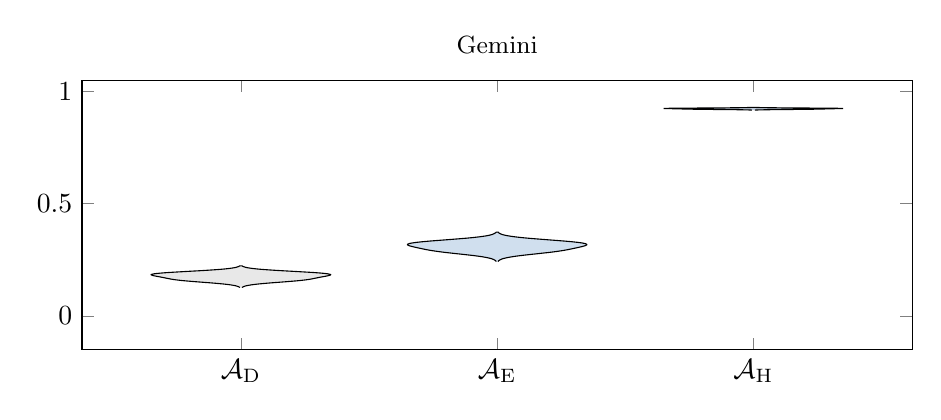
\begin{tikzpicture}
\begin{axis}[width=\textwidth, height=5cm, ymin=-0.15, ymax=1.05,
  xtick={1,2,3}, xticklabels={$\mathcal{A}_{\text{D}}$,$\mathcal{A}_{\text{E}}$,$\mathcal{A}_{\text{H}}$},
  title={\small Gemini}, title style={font=\small}]
\addplot[no marks, fill=colorPure!60, fill opacity=0.5] coordinates { (1.0043,0.1261) (1.0067,0.1281) (1.0100,0.1300) (1.0147,0.1320) (1.0210,0.1340) (1.0293,0.1359) (1.0398,0.1379) (1.0528,0.1399) (1.0683,0.1419) (1.0861,0.1438) (1.1061,0.1458) (1.1277,0.1478) (1.1502,0.1497) (1.1727,0.1517) (1.1944,0.1537) (1.2145,0.1556) (1.2324,0.1576) (1.2479,0.1596) (1.2609,0.1615) (1.2717,0.1635) (1.2809,0.1655) (1.2893,0.1675) (1.2976,0.1694) (1.3062,0.1714) (1.3153,0.1734) (1.3248,0.1753) (1.3341,0.1773) (1.3422,0.1793) (1.3479,0.1812) (1.3500,0.1832) (1.3474,0.1852) (1.3394,0.1872) (1.3257,0.1891) (1.3065,0.1911) (1.2825,0.1931) (1.2547,0.1950) (1.2246,0.1970) (1.1935,0.1990) (1.1628,0.2009) (1.1338,0.2029) (1.1073,0.2049) (1.0840,0.2068) (1.0642,0.2088) (1.0479,0.2108) (1.0348,0.2128) (1.0247,0.2147) (1.0171,0.2167) (1.0116,0.2187) (1.0076,0.2206) (1.0049,0.2226) (0.9951,0.2226) (0.9924,0.2206) (0.9884,0.2187) (0.9829,0.2167) (0.9753,0.2147) (0.9652,0.2128) (0.9521,0.2108) (0.9358,0.2088) (0.9160,0.2068) (0.8927,0.2049) (0.8662,0.2029) (0.8372,0.2009) (0.8065,0.1990) (0.7754,0.1970) (0.7453,0.1950) (0.7175,0.1931) (0.6935,0.1911) (0.6743,0.1891) (0.6606,0.1872) (0.6526,0.1852) (0.6500,0.1832) (0.6521,0.1812) (0.6578,0.1793) (0.6659,0.1773) (0.6752,0.1753) (0.6847,0.1734) (0.6938,0.1714) (0.7024,0.1694) (0.7107,0.1675) (0.7191,0.1655) (0.7283,0.1635) (0.7391,0.1615) (0.7521,0.1596) (0.7676,0.1576) (0.7855,0.1556) (0.8056,0.1537) (0.8273,0.1517) (0.8498,0.1497) (0.8723,0.1478) (0.8939,0.1458) (0.9139,0.1438) (0.9317,0.1419) (0.9472,0.1399) (0.9602,0.1379) (0.9707,0.1359) (0.9790,0.1340) (0.9853,0.1320) (0.9900,0.1300) (0.9933,0.1281) (0.9957,0.1261) };
\addplot[no marks, fill=colorRAG!60, fill opacity=0.5] coordinates { (2.0034,0.2420) (2.0053,0.2447) (2.0081,0.2473) (2.0120,0.2500) (2.0173,0.2527) (2.0244,0.2554) (2.0336,0.2580) (2.0450,0.2607) (2.0588,0.2634) (2.0749,0.2661) (2.0932,0.2688) (2.1133,0.2714) (2.1347,0.2741) (2.1565,0.2768) (2.1782,0.2795) (2.1990,0.2821) (2.2183,0.2848) (2.2359,0.2875) (2.2515,0.2902) (2.2654,0.2928) (2.2779,0.2955) (2.2895,0.2982) (2.3006,0.3009) (2.3114,0.3035) (2.3219,0.3062) (2.3318,0.3089) (2.3404,0.3116) (2.3469,0.3142) (2.3500,0.3169) (2.3489,0.3196) (2.3427,0.3223) (2.3311,0.3249) (2.3139,0.3276) (2.2918,0.3303) (2.2656,0.3330) (2.2366,0.3356) (2.2060,0.3383) (2.1752,0.3410) (2.1456,0.3437) (2.1181,0.3463) (2.0936,0.3490) (2.0724,0.3517) (2.0546,0.3544) (2.0402,0.3571) (2.0289,0.3597) (2.0202,0.3624) (2.0138,0.3651) (2.0092,0.3678) (2.0060,0.3704) (2.0038,0.3731) (1.9962,0.3731) (1.9940,0.3704) (1.9908,0.3678) (1.9862,0.3651) (1.9798,0.3624) (1.9711,0.3597) (1.9598,0.3571) (1.9454,0.3544) (1.9276,0.3517) (1.9064,0.3490) (1.8819,0.3463) (1.8544,0.3437) (1.8248,0.3410) (1.7940,0.3383) (1.7634,0.3356) (1.7344,0.3330) (1.7082,0.3303) (1.6861,0.3276) (1.6689,0.3249) (1.6573,0.3223) (1.6511,0.3196) (1.6500,0.3169) (1.6531,0.3142) (1.6596,0.3116) (1.6682,0.3089) (1.6781,0.3062) (1.6886,0.3035) (1.6994,0.3009) (1.7105,0.2982) (1.7221,0.2955) (1.7346,0.2928) (1.7485,0.2902) (1.7641,0.2875) (1.7817,0.2848) (1.8010,0.2821) (1.8218,0.2795) (1.8435,0.2768) (1.8653,0.2741) (1.8867,0.2714) (1.9068,0.2688) (1.9251,0.2661) (1.9412,0.2634) (1.9550,0.2607) (1.9664,0.2580) (1.9756,0.2554) (1.9827,0.2527) (1.9880,0.2500) (1.9919,0.2473) (1.9947,0.2447) (1.9966,0.2420) };
\addplot[no marks, fill=colorLLMParameterizedReferenceScoring!60, fill opacity=0.5] coordinates { (3.0059,0.9171) (3.0088,0.9174) (3.0128,0.9176) (3.0181,0.9178) (3.0252,0.9181) (3.0342,0.9183) (3.0454,0.9186) (3.0589,0.9188) (3.0746,0.9191) (3.0924,0.9193) (3.1120,0.9196) (3.1327,0.9198) (3.1540,0.9200) (3.1749,0.9203) (3.1949,0.9205) (3.2130,0.9208) (3.2290,0.9210) (3.2425,0.9213) (3.2536,0.9215) (3.2626,0.9218) (3.2702,0.9220) (3.2772,0.9222) (3.2843,0.9225) (3.2921,0.9227) (3.3009,0.9230) (3.3108,0.9232) (3.3214,0.9235) (3.3317,0.9237) (3.3408,0.9240) (3.3473,0.9242) (3.3500,0.9244) (3.3479,0.9247) (3.3403,0.9249) (3.3270,0.9252) (3.3082,0.9254) (3.2846,0.9257) (3.2574,0.9259) (3.2277,0.9262) (3.1971,0.9264) (3.1668,0.9266) (3.1379,0.9269) (3.1115,0.9271) (3.0881,0.9274) (3.0680,0.9276) (3.0513,0.9279) (3.0378,0.9281) (3.0272,0.9284) (3.0191,0.9286) (3.0131,0.9288) (3.0088,0.9291) (2.9912,0.9291) (2.9869,0.9288) (2.9809,0.9286) (2.9728,0.9284) (2.9622,0.9281) (2.9487,0.9279) (2.9320,0.9276) (2.9119,0.9274) (2.8885,0.9271) (2.8621,0.9269) (2.8332,0.9266) (2.8029,0.9264) (2.7723,0.9262) (2.7426,0.9259) (2.7154,0.9257) (2.6918,0.9254) (2.6730,0.9252) (2.6597,0.9249) (2.6521,0.9247) (2.6500,0.9244) (2.6527,0.9242) (2.6592,0.9240) (2.6683,0.9237) (2.6786,0.9235) (2.6892,0.9232) (2.6991,0.9230) (2.7079,0.9227) (2.7157,0.9225) (2.7228,0.9222) (2.7298,0.9220) (2.7374,0.9218) (2.7464,0.9215) (2.7575,0.9213) (2.7710,0.9210) (2.7870,0.9208) (2.8051,0.9205) (2.8251,0.9203) (2.8460,0.9200) (2.8673,0.9198) (2.8880,0.9196) (2.9076,0.9193) (2.9254,0.9191) (2.9411,0.9188) (2.9546,0.9186) (2.9658,0.9183) (2.9748,0.9181) (2.9819,0.9178) (2.9872,0.9176) (2.9912,0.9174) (2.9941,0.9171) };
\end{axis}
\end{tikzpicture}
\end{minipage}
\hfill
\begin{minipage}{0.24\textwidth}
\centering
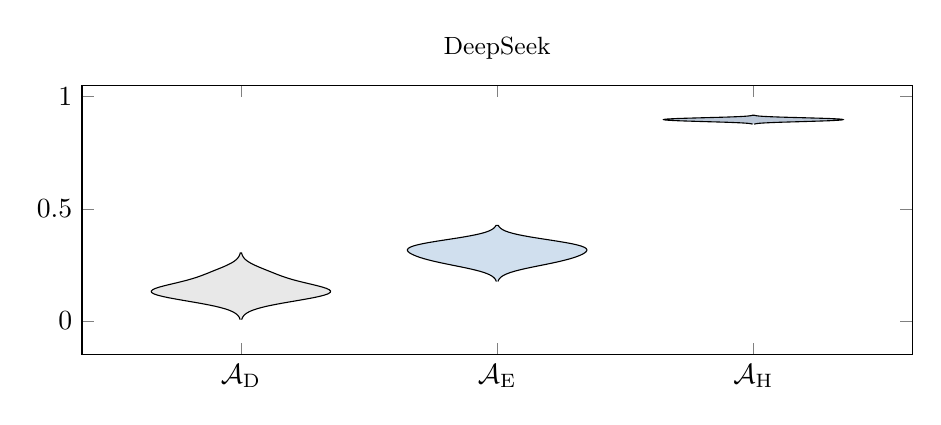
\begin{tikzpicture}
\begin{axis}[width=\textwidth, height=5cm, ymin=-0.15, ymax=1.05,
  xtick={1,2,3}, xticklabels={$\mathcal{A}_{\text{D}}$,$\mathcal{A}_{\text{E}}$,$\mathcal{A}_{\text{H}}$},
  title={\small DeepSeek}, title style={font=\small}]
\addplot[no marks, fill=colorPure!60, fill opacity=0.5] coordinates { (1.0030,0.0058) (1.0049,0.0119) (1.0076,0.0180) (1.0115,0.0240) (1.0170,0.0301) (1.0245,0.0362) (1.0344,0.0422) (1.0471,0.0483) (1.0629,0.0543) (1.0821,0.0604) (1.1046,0.0665) (1.1303,0.0725) (1.1586,0.0786) (1.1888,0.0846) (1.2199,0.0907) (1.2505,0.0968) (1.2792,0.1028) (1.3047,0.1089) (1.3254,0.1150) (1.3403,0.1210) (1.3486,0.1271) (1.3500,0.1331) (1.3447,0.1392) (1.3333,0.1453) (1.3170,0.1513) (1.2971,0.1574) (1.2753,0.1634) (1.2528,0.1695) (1.2309,0.1756) (1.2104,0.1816) (1.1917,0.1877) (1.1748,0.1937) (1.1595,0.1998) (1.1453,0.2059) (1.1318,0.2119) (1.1186,0.2180) (1.1054,0.2241) (1.0922,0.2301) (1.0791,0.2362) (1.0665,0.2422) (1.0545,0.2483) (1.0436,0.2544) (1.0340,0.2604) (1.0258,0.2665) (1.0190,0.2725) (1.0136,0.2786) (1.0095,0.2847) (1.0064,0.2907) (1.0042,0.2968) (1.0027,0.3029) (0.9973,0.3029) (0.9958,0.2968) (0.9936,0.2907) (0.9905,0.2847) (0.9864,0.2786) (0.9810,0.2725) (0.9742,0.2665) (0.9660,0.2604) (0.9564,0.2544) (0.9455,0.2483) (0.9335,0.2422) (0.9209,0.2362) (0.9078,0.2301) (0.8946,0.2241) (0.8814,0.2180) (0.8682,0.2119) (0.8547,0.2059) (0.8405,0.1998) (0.8252,0.1937) (0.8083,0.1877) (0.7896,0.1816) (0.7691,0.1756) (0.7472,0.1695) (0.7247,0.1634) (0.7029,0.1574) (0.6830,0.1513) (0.6667,0.1453) (0.6553,0.1392) (0.6500,0.1331) (0.6514,0.1271) (0.6597,0.1210) (0.6746,0.1150) (0.6953,0.1089) (0.7208,0.1028) (0.7495,0.0968) (0.7801,0.0907) (0.8112,0.0846) (0.8414,0.0786) (0.8697,0.0725) (0.8954,0.0665) (0.9179,0.0604) (0.9371,0.0543) (0.9529,0.0483) (0.9656,0.0422) (0.9755,0.0362) (0.9830,0.0301) (0.9885,0.0240) (0.9924,0.0180) (0.9951,0.0119) (0.9970,0.0058) };
\addplot[no marks, fill=colorRAG!60, fill opacity=0.5] coordinates { (2.0032,0.1759) (2.0049,0.1810) (2.0075,0.1861) (2.0111,0.1912) (2.0159,0.1963) (2.0224,0.2014) (2.0307,0.2065) (2.0411,0.2116) (2.0537,0.2167) (2.0685,0.2218) (2.0856,0.2269) (2.1045,0.2320) (2.1250,0.2371) (2.1466,0.2422) (2.1688,0.2473) (2.1910,0.2524) (2.2127,0.2575) (2.2333,0.2626) (2.2527,0.2677) (2.2704,0.2728) (2.2865,0.2779) (2.3009,0.2830) (2.3136,0.2881) (2.3247,0.2932) (2.3341,0.2983) (2.3416,0.3034) (2.3470,0.3085) (2.3500,0.3136) (2.3500,0.3187) (2.3465,0.3238) (2.3391,0.3289) (2.3275,0.3340) (2.3116,0.3391) (2.2916,0.3442) (2.2679,0.3493) (2.2414,0.3544) (2.2131,0.3595) (2.1841,0.3646) (2.1554,0.3697) (2.1282,0.3748) (2.1033,0.3799) (2.0811,0.3850) (2.0622,0.3901) (2.0464,0.3952) (2.0338,0.4003) (2.0240,0.4054) (2.0166,0.4105) (2.0112,0.4156) (2.0073,0.4207) (2.0047,0.4258) (1.9953,0.4258) (1.9927,0.4207) (1.9888,0.4156) (1.9834,0.4105) (1.9760,0.4054) (1.9662,0.4003) (1.9536,0.3952) (1.9378,0.3901) (1.9189,0.3850) (1.8967,0.3799) (1.8718,0.3748) (1.8446,0.3697) (1.8159,0.3646) (1.7869,0.3595) (1.7586,0.3544) (1.7321,0.3493) (1.7084,0.3442) (1.6884,0.3391) (1.6725,0.3340) (1.6609,0.3289) (1.6535,0.3238) (1.6500,0.3187) (1.6500,0.3136) (1.6530,0.3085) (1.6584,0.3034) (1.6659,0.2983) (1.6753,0.2932) (1.6864,0.2881) (1.6991,0.2830) (1.7135,0.2779) (1.7296,0.2728) (1.7473,0.2677) (1.7667,0.2626) (1.7873,0.2575) (1.8090,0.2524) (1.8312,0.2473) (1.8534,0.2422) (1.8750,0.2371) (1.8955,0.2320) (1.9144,0.2269) (1.9315,0.2218) (1.9463,0.2167) (1.9589,0.2116) (1.9693,0.2065) (1.9776,0.2014) (1.9841,0.1963) (1.9889,0.1912) (1.9925,0.1861) (1.9951,0.1810) (1.9968,0.1759) };
\addplot[no marks, fill=colorLLMParameterizedReferenceScoring!60, fill opacity=0.5] coordinates { (3.0032,0.8771) (3.0051,0.8779) (3.0078,0.8787) (3.0116,0.8795) (3.0168,0.8803) (3.0238,0.8812) (3.0329,0.8820) (3.0442,0.8828) (3.0581,0.8836) (3.0745,0.8844) (3.0933,0.8853) (3.1144,0.8861) (3.1372,0.8869) (3.1613,0.8877) (3.1859,0.8885) (3.2105,0.8894) (3.2344,0.8902) (3.2569,0.8910) (3.2775,0.8918) (3.2960,0.8926) (3.3119,0.8935) (3.3252,0.8943) (3.3357,0.8951) (3.3434,0.8959) (3.3482,0.8967) (3.3500,0.8976) (3.3488,0.8984) (3.3444,0.8992) (3.3367,0.9000) (3.3257,0.9008) (3.3114,0.9017) (3.2939,0.9025) (3.2734,0.9033) (3.2505,0.9041) (3.2257,0.9049) (3.1997,0.9058) (3.1733,0.9066) (3.1475,0.9074) (3.1228,0.9082) (3.1001,0.9090) (3.0797,0.9099) (3.0620,0.9107) (3.0471,0.9115) (3.0349,0.9123) (3.0252,0.9131) (3.0177,0.9140) (3.0122,0.9148) (3.0081,0.9156) (3.0053,0.9164) (3.0033,0.9172) (2.9967,0.9172) (2.9947,0.9164) (2.9919,0.9156) (2.9878,0.9148) (2.9823,0.9140) (2.9748,0.9131) (2.9651,0.9123) (2.9529,0.9115) (2.9380,0.9107) (2.9203,0.9099) (2.8999,0.9090) (2.8772,0.9082) (2.8525,0.9074) (2.8267,0.9066) (2.8003,0.9058) (2.7743,0.9049) (2.7495,0.9041) (2.7266,0.9033) (2.7061,0.9025) (2.6886,0.9017) (2.6743,0.9008) (2.6633,0.9000) (2.6556,0.8992) (2.6512,0.8984) (2.6500,0.8976) (2.6518,0.8967) (2.6566,0.8959) (2.6643,0.8951) (2.6748,0.8943) (2.6881,0.8935) (2.7040,0.8926) (2.7225,0.8918) (2.7431,0.8910) (2.7656,0.8902) (2.7895,0.8894) (2.8141,0.8885) (2.8387,0.8877) (2.8628,0.8869) (2.8856,0.8861) (2.9067,0.8853) (2.9255,0.8844) (2.9419,0.8836) (2.9558,0.8828) (2.9671,0.8820) (2.9762,0.8812) (2.9832,0.8803) (2.9884,0.8795) (2.9922,0.8787) (2.9949,0.8779) (2.9968,0.8771) };
\end{axis}
\end{tikzpicture}
\end{minipage}
\hfill
\begin{minipage}{0.24\textwidth}
\centering
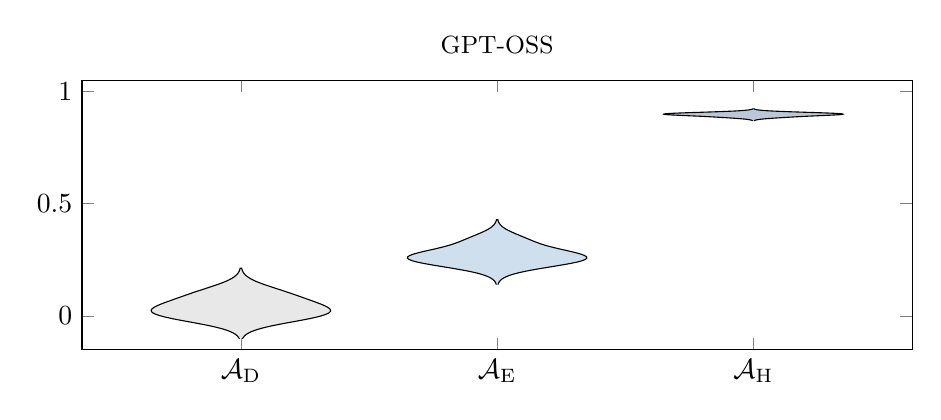
\begin{tikzpicture}
\begin{axis}[width=\textwidth, height=5cm, ymin=-0.15, ymax=1.05,
  xtick={1,2,3}, xticklabels={$\mathcal{A}_{\text{D}}$,$\mathcal{A}_{\text{E}}$,$\mathcal{A}_{\text{H}}$},
  title={\small GPT-OSS}, title style={font=\small}]
\addplot[no marks, fill=colorPure!60, fill opacity=0.5] coordinates { (1.0060,-0.1025) (1.0093,-0.0961) (1.0140,-0.0896) (1.0206,-0.0832) (1.0294,-0.0768) (1.0411,-0.0704) (1.0558,-0.0640) (1.0739,-0.0576) (1.0955,-0.0512) (1.1204,-0.0447) (1.1480,-0.0383) (1.1777,-0.0319) (1.2083,-0.0255) (1.2387,-0.0191) (1.2675,-0.0127) (1.2933,-0.0062) (1.3151,0.0002) (1.3320,0.0066) (1.3434,0.0130) (1.3494,0.0194) (1.3500,0.0258) (1.3459,0.0322) (1.3379,0.0387) (1.3269,0.0451) (1.3137,0.0515) (1.2991,0.0579) (1.2838,0.0643) (1.2681,0.0707) (1.2523,0.0772) (1.2365,0.0836) (1.2206,0.0900) (1.2046,0.0964) (1.1882,0.1028) (1.1714,0.1092) (1.1543,0.1156) (1.1370,0.1221) (1.1198,0.1285) (1.1029,0.1349) (1.0867,0.1413) (1.0716,0.1477) (1.0579,0.1541) (1.0458,0.1606) (1.0354,0.1670) (1.0267,0.1734) (1.0196,0.1798) (1.0141,0.1862) (1.0099,0.1926) (1.0067,0.1990) (1.0045,0.2055) (1.0029,0.2119) (0.9971,0.2119) (0.9955,0.2055) (0.9933,0.1990) (0.9901,0.1926) (0.9859,0.1862) (0.9804,0.1798) (0.9733,0.1734) (0.9646,0.1670) (0.9542,0.1606) (0.9421,0.1541) (0.9284,0.1477) (0.9133,0.1413) (0.8971,0.1349) (0.8802,0.1285) (0.8630,0.1221) (0.8457,0.1156) (0.8286,0.1092) (0.8118,0.1028) (0.7954,0.0964) (0.7794,0.0900) (0.7635,0.0836) (0.7477,0.0772) (0.7319,0.0707) (0.7162,0.0643) (0.7009,0.0579) (0.6863,0.0515) (0.6731,0.0451) (0.6621,0.0387) (0.6541,0.0322) (0.6500,0.0258) (0.6506,0.0194) (0.6566,0.0130) (0.6680,0.0066) (0.6849,0.0002) (0.7067,-0.0062) (0.7325,-0.0127) (0.7613,-0.0191) (0.7917,-0.0255) (0.8223,-0.0319) (0.8520,-0.0383) (0.8796,-0.0447) (0.9045,-0.0512) (0.9261,-0.0576) (0.9442,-0.0640) (0.9589,-0.0704) (0.9706,-0.0768) (0.9794,-0.0832) (0.9860,-0.0896) (0.9907,-0.0961) (0.9940,-0.1025) };
\addplot[no marks, fill=colorRAG!60, fill opacity=0.5] coordinates { (2.0031,0.1391) (2.0050,0.1451) (2.0078,0.1510) (2.0118,0.1569) (2.0175,0.1628) (2.0252,0.1687) (2.0355,0.1746) (2.0487,0.1805) (2.0652,0.1864) (2.0852,0.1923) (2.1086,0.1982) (2.1353,0.2041) (2.1646,0.2100) (2.1957,0.2159) (2.2274,0.2218) (2.2583,0.2277) (2.2868,0.2336) (2.3115,0.2395) (2.3309,0.2454) (2.3440,0.2513) (2.3500,0.2572) (2.3489,0.2631) (2.3410,0.2690) (2.3272,0.2749) (2.3089,0.2808) (2.2876,0.2868) (2.2648,0.2927) (2.2419,0.2986) (2.2202,0.3045) (2.2003,0.3104) (2.1824,0.3163) (2.1666,0.3222) (2.1524,0.3281) (2.1394,0.3340) (2.1269,0.3399) (2.1146,0.3458) (2.1022,0.3517) (2.0896,0.3576) (2.0771,0.3635) (2.0649,0.3694) (2.0534,0.3753) (2.0428,0.3812) (2.0334,0.3871) (2.0253,0.3930) (2.0187,0.3989) (2.0134,0.4048) (2.0093,0.4107) (2.0063,0.4166) (2.0041,0.4225) (2.0026,0.4285) (1.9974,0.4285) (1.9959,0.4225) (1.9937,0.4166) (1.9907,0.4107) (1.9866,0.4048) (1.9813,0.3989) (1.9747,0.3930) (1.9666,0.3871) (1.9572,0.3812) (1.9466,0.3753) (1.9351,0.3694) (1.9229,0.3635) (1.9104,0.3576) (1.8978,0.3517) (1.8854,0.3458) (1.8731,0.3399) (1.8606,0.3340) (1.8476,0.3281) (1.8334,0.3222) (1.8176,0.3163) (1.7997,0.3104) (1.7798,0.3045) (1.7581,0.2986) (1.7352,0.2927) (1.7124,0.2868) (1.6911,0.2808) (1.6728,0.2749) (1.6590,0.2690) (1.6511,0.2631) (1.6500,0.2572) (1.6560,0.2513) (1.6691,0.2454) (1.6885,0.2395) (1.7132,0.2336) (1.7417,0.2277) (1.7726,0.2218) (1.8043,0.2159) (1.8354,0.2100) (1.8647,0.2041) (1.8914,0.1982) (1.9148,0.1923) (1.9348,0.1864) (1.9513,0.1805) (1.9645,0.1746) (1.9748,0.1687) (1.9825,0.1628) (1.9882,0.1569) (1.9922,0.1510) (1.9950,0.1451) (1.9969,0.1391) };
\addplot[no marks, fill=colorLLMParameterizedReferenceScoring!60, fill opacity=0.5] coordinates { (3.0027,0.8696) (3.0043,0.8707) (3.0066,0.8718) (3.0098,0.8729) (3.0141,0.8740) (3.0197,0.8750) (3.0268,0.8761) (3.0354,0.8772) (3.0456,0.8783) (3.0573,0.8794) (3.0702,0.8804) (3.0840,0.8815) (3.0986,0.8826) (3.1137,0.8837) (3.1292,0.8848) (3.1451,0.8858) (3.1616,0.8869) (3.1789,0.8880) (3.1973,0.8891) (3.2170,0.8902) (3.2378,0.8912) (3.2593,0.8923) (3.2809,0.8934) (3.3015,0.8945) (3.3199,0.8956) (3.3348,0.8966) (3.3451,0.8977) (3.3500,0.8988) (3.3488,0.8999) (3.3415,0.9010) (3.3283,0.9020) (3.3099,0.9031) (3.2872,0.9042) (3.2612,0.9053) (3.2332,0.9064) (3.2042,0.9074) (3.1754,0.9085) (3.1476,0.9096) (3.1217,0.9107) (3.0982,0.9118) (3.0775,0.9128) (3.0598,0.9139) (3.0450,0.9150) (3.0331,0.9161) (3.0237,0.9172) (3.0166,0.9182) (3.0113,0.9193) (3.0075,0.9204) (3.0048,0.9215) (3.0030,0.9226) (2.9970,0.9226) (2.9952,0.9215) (2.9925,0.9204) (2.9887,0.9193) (2.9834,0.9182) (2.9763,0.9172) (2.9669,0.9161) (2.9550,0.9150) (2.9402,0.9139) (2.9225,0.9128) (2.9018,0.9118) (2.8783,0.9107) (2.8524,0.9096) (2.8246,0.9085) (2.7958,0.9074) (2.7668,0.9064) (2.7388,0.9053) (2.7128,0.9042) (2.6901,0.9031) (2.6717,0.9020) (2.6585,0.9010) (2.6512,0.8999) (2.6500,0.8988) (2.6549,0.8977) (2.6652,0.8966) (2.6801,0.8956) (2.6985,0.8945) (2.7191,0.8934) (2.7407,0.8923) (2.7622,0.8912) (2.7830,0.8902) (2.8027,0.8891) (2.8211,0.8880) (2.8384,0.8869) (2.8549,0.8858) (2.8708,0.8848) (2.8863,0.8837) (2.9014,0.8826) (2.9160,0.8815) (2.9298,0.8804) (2.9427,0.8794) (2.9544,0.8783) (2.9646,0.8772) (2.9732,0.8761) (2.9803,0.8750) (2.9859,0.8740) (2.9902,0.8729) (2.9934,0.8718) (2.9957,0.8707) (2.9973,0.8696) };
\end{axis}
\end{tikzpicture}
\end{minipage}
\hfill
\begin{minipage}{0.24\textwidth}
\centering
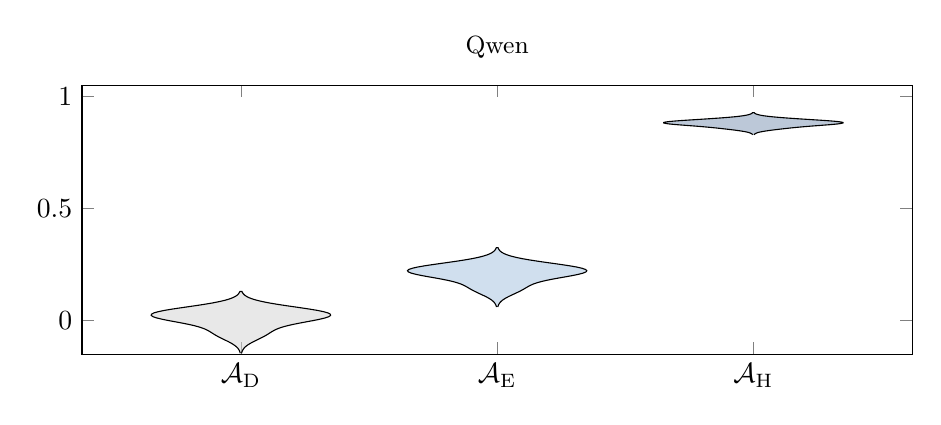
\begin{tikzpicture}
\begin{axis}[width=\textwidth, height=5cm, ymin=-0.15, ymax=1.05,
  xtick={1,2,3}, xticklabels={$\mathcal{A}_{\text{D}}$,$\mathcal{A}_{\text{E}}$,$\mathcal{A}_{\text{H}}$},
  title={\small Qwen}, title style={font=\small}]
\addplot[no marks, fill=colorPure!60, fill opacity=0.5] coordinates { (1.0025,-0.1452) (1.0039,-0.1396) (1.0058,-0.1340) (1.0086,-0.1283) (1.0122,-0.1227) (1.0169,-0.1171) (1.0228,-0.1115) (1.0299,-0.1059) (1.0382,-0.1003) (1.0473,-0.0946) (1.0572,-0.0890) (1.0673,-0.0834) (1.0774,-0.0778) (1.0871,-0.0722) (1.0960,-0.0666) (1.1043,-0.0610) (1.1121,-0.0553) (1.1199,-0.0497) (1.1283,-0.0441) (1.1382,-0.0385) (1.1505,-0.0329) (1.1658,-0.0273) (1.1845,-0.0216) (1.2065,-0.0160) (1.2312,-0.0104) (1.2574,-0.0048) (1.2837,0.0008) (1.3079,0.0064) (1.3283,0.0121) (1.3428,0.0177) (1.3500,0.0233) (1.3490,0.0289) (1.3397,0.0345) (1.3224,0.0401) (1.2983,0.0458) (1.2691,0.0514) (1.2365,0.0570) (1.2025,0.0626) (1.1689,0.0682) (1.1373,0.0738) (1.1087,0.0794) (1.0838,0.0851) (1.0629,0.0907) (1.0460,0.0963) (1.0328,0.1019) (1.0227,0.1075) (1.0153,0.1131) (1.0101,0.1188) (1.0065,0.1244) (1.0040,0.1300) (0.9960,0.1300) (0.9935,0.1244) (0.9899,0.1188) (0.9847,0.1131) (0.9773,0.1075) (0.9672,0.1019) (0.9540,0.0963) (0.9371,0.0907) (0.9162,0.0851) (0.8913,0.0794) (0.8627,0.0738) (0.8311,0.0682) (0.7975,0.0626) (0.7635,0.0570) (0.7309,0.0514) (0.7017,0.0458) (0.6776,0.0401) (0.6603,0.0345) (0.6510,0.0289) (0.6500,0.0233) (0.6572,0.0177) (0.6717,0.0121) (0.6921,0.0064) (0.7163,0.0008) (0.7426,-0.0048) (0.7688,-0.0104) (0.7935,-0.0160) (0.8155,-0.0216) (0.8342,-0.0273) (0.8495,-0.0329) (0.8618,-0.0385) (0.8717,-0.0441) (0.8801,-0.0497) (0.8879,-0.0553) (0.8957,-0.0610) (0.9040,-0.0666) (0.9129,-0.0722) (0.9226,-0.0778) (0.9327,-0.0834) (0.9428,-0.0890) (0.9527,-0.0946) (0.9618,-0.1003) (0.9701,-0.1059) (0.9772,-0.1115) (0.9831,-0.1171) (0.9878,-0.1227) (0.9914,-0.1283) (0.9942,-0.1340) (0.9961,-0.1396) (0.9975,-0.1452) };
\addplot[no marks, fill=colorRAG!60, fill opacity=0.5] coordinates { (2.0025,0.0609) (2.0039,0.0663) (2.0059,0.0717) (2.0087,0.0771) (2.0124,0.0825) (2.0173,0.0879) (2.0233,0.0933) (2.0306,0.0987) (2.0390,0.1041) (2.0483,0.1095) (2.0583,0.1149) (2.0686,0.1203) (2.0787,0.1257) (2.0884,0.1311) (2.0974,0.1365) (2.1058,0.1419) (2.1137,0.1473) (2.1219,0.1527) (2.1310,0.1581) (2.1419,0.1635) (2.1555,0.1689) (2.1723,0.1743) (2.1926,0.1797) (2.2162,0.1851) (2.2420,0.1905) (2.2688,0.1958) (2.2946,0.2012) (2.3175,0.2066) (2.3354,0.2120) (2.3467,0.2174) (2.3500,0.2228) (2.3449,0.2282) (2.3314,0.2336) (2.3106,0.2390) (2.2837,0.2444) (2.2526,0.2498) (2.2193,0.2552) (2.1855,0.2606) (2.1530,0.2660) (2.1230,0.2714) (2.0963,0.2768) (2.0736,0.2822) (2.0548,0.2876) (2.0397,0.2930) (2.0281,0.2984) (2.0193,0.3038) (2.0130,0.3092) (2.0085,0.3146) (2.0054,0.3200) (2.0034,0.3254) (1.9966,0.3254) (1.9946,0.3200) (1.9915,0.3146) (1.9870,0.3092) (1.9807,0.3038) (1.9719,0.2984) (1.9603,0.2930) (1.9452,0.2876) (1.9264,0.2822) (1.9037,0.2768) (1.8770,0.2714) (1.8470,0.2660) (1.8145,0.2606) (1.7807,0.2552) (1.7474,0.2498) (1.7163,0.2444) (1.6894,0.2390) (1.6686,0.2336) (1.6551,0.2282) (1.6500,0.2228) (1.6533,0.2174) (1.6646,0.2120) (1.6825,0.2066) (1.7054,0.2012) (1.7312,0.1958) (1.7580,0.1905) (1.7838,0.1851) (1.8074,0.1797) (1.8277,0.1743) (1.8445,0.1689) (1.8581,0.1635) (1.8690,0.1581) (1.8781,0.1527) (1.8863,0.1473) (1.8942,0.1419) (1.9026,0.1365) (1.9116,0.1311) (1.9213,0.1257) (1.9314,0.1203) (1.9417,0.1149) (1.9517,0.1095) (1.9610,0.1041) (1.9694,0.0987) (1.9767,0.0933) (1.9827,0.0879) (1.9876,0.0825) (1.9913,0.0771) (1.9941,0.0717) (1.9961,0.0663) (1.9975,0.0609) };
\addplot[no marks, fill=colorLLMParameterizedReferenceScoring!60, fill opacity=0.5] coordinates { (3.0027,0.8291) (3.0043,0.8311) (3.0066,0.8331) (3.0098,0.8352) (3.0142,0.8372) (3.0199,0.8392) (3.0270,0.8412) (3.0358,0.8432) (3.0461,0.8452) (3.0579,0.8472) (3.0709,0.8492) (3.0850,0.8512) (3.0998,0.8532) (3.1152,0.8552) (3.1311,0.8573) (3.1477,0.8593) (3.1652,0.8613) (3.1839,0.8633) (3.2039,0.8653) (3.2254,0.8673) (3.2480,0.8693) (3.2710,0.8713) (3.2935,0.8733) (3.3139,0.8753) (3.3310,0.8773) (3.3434,0.8794) (3.3499,0.8814) (3.3500,0.8834) (3.3435,0.8854) (3.3308,0.8874) (3.3128,0.8894) (3.2905,0.8914) (3.2652,0.8934) (3.2380,0.8954) (3.2102,0.8974) (3.1826,0.8994) (3.1559,0.9015) (3.1309,0.9035) (3.1079,0.9055) (3.0873,0.9075) (3.0691,0.9095) (3.0536,0.9115) (3.0406,0.9135) (3.0300,0.9155) (3.0217,0.9175) (3.0152,0.9195) (3.0104,0.9215) (3.0069,0.9236) (3.0045,0.9256) (3.0028,0.9276) (2.9972,0.9276) (2.9955,0.9256) (2.9931,0.9236) (2.9896,0.9215) (2.9848,0.9195) (2.9783,0.9175) (2.9700,0.9155) (2.9594,0.9135) (2.9464,0.9115) (2.9309,0.9095) (2.9127,0.9075) (2.8921,0.9055) (2.8691,0.9035) (2.8441,0.9015) (2.8174,0.8994) (2.7898,0.8974) (2.7620,0.8954) (2.7348,0.8934) (2.7095,0.8914) (2.6872,0.8894) (2.6692,0.8874) (2.6565,0.8854) (2.6500,0.8834) (2.6501,0.8814) (2.6566,0.8794) (2.6690,0.8773) (2.6861,0.8753) (2.7065,0.8733) (2.7290,0.8713) (2.7520,0.8693) (2.7746,0.8673) (2.7961,0.8653) (2.8161,0.8633) (2.8348,0.8613) (2.8523,0.8593) (2.8689,0.8573) (2.8848,0.8552) (2.9002,0.8532) (2.9150,0.8512) (2.9291,0.8492) (2.9421,0.8472) (2.9539,0.8452) (2.9642,0.8432) (2.9730,0.8412) (2.9801,0.8392) (2.9858,0.8372) (2.9902,0.8352) (2.9934,0.8331) (2.9957,0.8311) (2.9973,0.8291) };
\end{axis}
\end{tikzpicture}
\end{minipage}
\caption{Violin plots of Kendall's $\tau$ across five runs.}
\end{threeparttable}
\label{fig:violin_tau}
\end{figure*}\subsection{Run-to-Run Variance: Full Distributions}
\label{app:variance}

\begin{figure*}[t]
\centering
\begin{minipage}{0.24\textwidth}
\centering
\begin{tikzpicture}
\begin{axis}[width=\textwidth, height=5cm, xmin=0.4, xmax=3.6, ymin=0, ymax=0.35,
  xtick={1,2,3}, xticklabels={$\mathcal{A}_{\text{D}}$,$\mathcal{A}_{\text{E}}$,$\mathcal{A}_{\text{H}}$},
  title={\small Gemini}, title style={font=\small}]
\addplot[only marks, mark=*, mark size=2pt, color=colorGemini] coordinates {
(0.92,0.2922) (0.96,0.2960) (1.00,0.2961) (1.04,0.2970) (1.08,0.2954)
(1.92,0.2327) (1.96,0.2307) (2.00,0.2312) (2.04,0.2283) (2.08,0.2328)
(2.92,0.0994) (2.96,0.0998) (3.00,0.1001) (3.04,0.1025) (3.08,0.1015)
};
\end{axis}
\end{tikzpicture}
\end{minipage}
\hfill
\begin{minipage}{0.24\textwidth}
\centering
\begin{tikzpicture}
\begin{axis}[width=\textwidth, height=5cm, xmin=0.4, xmax=3.6, ymin=0, ymax=0.35,
  xtick={1,2,3}, xticklabels={$\mathcal{A}_{\text{D}}$,$\mathcal{A}_{\text{E}}$,$\mathcal{A}_{\text{H}}$},
  title={\small DeepSeek}, title style={font=\small}]
\addplot[only marks, mark=*, mark size=2pt, color=colorDeepSeek] coordinates {
(0.92,0.3016) (0.96,0.3008) (1.00,0.3070) (1.04,0.2987) (1.08,0.3006)
(1.92,0.2376) (1.96,0.2346) (2.00,0.2366) (2.04,0.2374) (2.08,0.2364)
(2.92,0.0781) (2.96,0.0957) (3.00,0.0943) (3.04,0.0839) (3.08,0.1066)
};
\end{axis}
\end{tikzpicture}
\end{minipage}
\hfill
\begin{minipage}{0.24\textwidth}
\centering
\begin{tikzpicture}
\begin{axis}[width=\textwidth, height=5cm, xmin=0.4, xmax=3.6, ymin=0, ymax=0.35,
  xtick={1,2,3}, xticklabels={$\mathcal{A}_{\text{D}}$,$\mathcal{A}_{\text{E}}$,$\mathcal{A}_{\text{H}}$},
  title={\small GPT-OSS}, title style={font=\small}]
\addplot[only marks, mark=*, mark size=2pt, color=colorGPTOSS] coordinates {
(0.92,0.3061) (0.96,0.3057) (1.00,0.3041) (1.04,0.3079) (1.08,0.3076)
(1.92,0.2445) (1.96,0.2435) (2.00,0.2373) (2.04,0.2448) (2.08,0.2407)
(2.92,0.0996) (2.96,0.1016) (3.00,0.1089) (3.04,0.0989) (3.08,0.0984)
};
\end{axis}
\end{tikzpicture}
\end{minipage}
\hfill
\begin{minipage}{0.24\textwidth}
\centering
\begin{tikzpicture}
\begin{axis}[width=\textwidth, height=5cm, xmin=0.4, xmax=3.6, ymin=0, ymax=0.35,
  xtick={1,2,3}, xticklabels={$\mathcal{A}_{\text{D}}$,$\mathcal{A}_{\text{E}}$,$\mathcal{A}_{\text{H}}$},
  title={\small Qwen}, title style={font=\small}]
\addplot[only marks, mark=*, mark size=2pt, color=colorQwen] coordinates {
(0.92,0.2980) (0.96,0.2945) (1.00,0.2930) (1.04,0.2942) (1.08,0.2943)
(1.92,0.2631) (1.96,0.2646) (2.00,0.2547) (2.04,0.2636) (2.08,0.2568)
(2.92,0.1661) (2.96,0.1570) (3.00,0.1633) (3.04,0.1666) (3.08,0.1574)
};
\end{axis}
\end{tikzpicture}
\end{minipage}
\caption{Strip plots of Overall RMSE across five runs.}
\label{fig:violin_rmse}
\end{figure*}

MAE and Top-1 distribution shapes across runs, and the per-model MAE breakdown, are omitted here because Table~\ref{tab:overall_by_model} (~\ref{app:numerical_results}) already reports mean $\pm$ std for every metric.\subsection{Statistical Significance Tests}
\label{app:significance}

All tests use per-scenario metrics computed from the 195 test scenarios, with five independent runs per architecture--model combination.

\subsection{Pairwise Wilcoxon Tests, Reported Per Model}

Wilcoxon signed-rank tests compare each pair of adjacent architectures ($\mathcal{A}_{\text{D}}$ vs.\ $\mathcal{A}_{\text{E}}$ and $\mathcal{A}_{\text{E}}$ vs.\ $\mathcal{A}_{\text{H}}$) on each of the three primary metrics ($\tau$, MAE, Top-1), applied within each of the four models. All 24 per-model comparisons remain significant under Holm correction, whether corrected across the 24 tests reported here or across the full 56-test family. The largest adjusted values are DeepSeek's and Gemini's $\mathcal{A}_{\text{D}}$ vs.\ $\mathcal{A}_{\text{E}}$ tests on $\tau$ (both $p_{\mathrm{Holm}} = 0.0062$) and Gemini's on Top-1 ($0.0036$); the other 21 fall at or below $1.6 \times 10^{-4}$, and the smallest is $5.2 \times 10^{-31}$. GPT-OSS contributes $n = 194$ rather than 195 on the $\mathcal{A}_{\text{E}}$ vs.\ $\mathcal{A}_{\text{H}}$ comparison, one scenario dropping from the paired set.

Two comparisons carry heavy tie loads, both of them Gemini's $\mathcal{A}_{\text{D}}$ vs.\ $\mathcal{A}_{\text{E}}$: 58 of 195 paired differences are exactly zero on $\tau$, and 102 of 195 on Top-1. Each reports a median paired difference of 0.0000 while the test stays significant, because the signed-rank statistic is computed over the non-tied pairs alone. Read Gemini's effect size for that comparison from Cliff's $\delta$ in Table~\ref{tab:effect_sizes} rather than from the median. Every test uses the asymptotic approximation with tie and continuity corrections; the exact method applies to no cell, since each either exceeds 25 non-zero pairs or carries ties. Per-test $Z$, median paired difference, tied-pair counts, and both Holm-corrected $p$-values are in \texttt{paper/per\_model\_pvalues.csv} in the repository.

\subsection{Effect Sizes}

Table~\ref{tab:effect_sizes} reports Cliff's $\delta$ for each pairwise comparison.

\begin{table}[t]
\centering
\begin{threeparttable}
\small
\centering
\renewcommand{\arraystretch}{1.10}
\caption{Cliff's $\delta$ effect sizes for pairwise architecture comparisons, shown per model.}
\label{tab:effect_sizes}
\begin{tabular}{@{}l l ccc@{}}
\toprule
Comparison & Model & $\tau$ & MAE & Top-1 \\
\midrule
\multirow{4}{*}{$\mathcal{A}_{\text{D}}$ vs.\ $\mathcal{A}_{\text{E}}$}
 & DeepSeek & $-$0.159 (small) & 0.494 (large) & $-$0.257 (small) \\
 & Gemini & $-$0.129 (negligible) & 0.400 (medium) & $-$0.157 (small) \\
 & GPT-OSS & $-$0.273 (small) & 0.489 (large) & $-$0.207 (small) \\
 & Qwen & $-$0.246 (small) & 0.319 (small) & $-$0.305 (small) \\
\midrule
\multirow{4}{*}{$\mathcal{A}_{\text{E}}$ vs.\ $\mathcal{A}_{\text{H}}$}
 & DeepSeek & $-$0.753 (large) & 0.884 (large) & $-$0.596 (large) \\
 & Gemini & $-$0.592 (large) & 0.778 (large) & $-$0.495 (large) \\
 & GPT-OSS & $-$0.780 (large) & 0.843 (large) & $-$0.661 (large) \\
 & Qwen & $-$0.835 (large) & 0.749 (large) & $-$0.721 (large) \\
\bottomrule
\end{tabular}
\renewcommand{\arraystretch}{1.0}
\end{threeparttable}
\end{table}

\subsection{Bootstrap Confidence Intervals}

Confidence intervals resample scenarios, not runs. Each of the 10,000 replicates draws 195 scenarios with replacement and carries all five runs of a drawn scenario together, so an interval covers the variation a different draw of households produces rather than the variation a different sampling seed produces. Scenarios are the unit a reader generalizes over, so the resampling treats them as the cluster. Table~\ref{tab:bootstrap_paired} reports paired architecture differences, drawing one scenario index and scoring both arms on it.

\begin{table}[t]
\centering
\begin{threeparttable}
\footnotesize
\centering
\setlength{\tabcolsep}{4pt}
\renewcommand{\arraystretch}{1.10}
\caption{Paired architecture differences from the same cluster bootstrap. Each replicate scores both architectures on one resampled scenario set, so the interval carries the correlation between the two arms.}
\label{tab:bootstrap_paired}
\begin{tabular}{@{}l l ccc@{}}
\toprule
Comparison & Model & $\tau$ & MAE & Top-1 (pp) \\
\midrule
\multirow{4}{*}{$\mathcal{A}_{\text{E}} - \mathcal{A}_{\text{D}}$}
 & DeepSeek & $+$0.163 [$+$0.070, $+$0.256] & $-$0.064 [$-$0.075, $-$0.052] & $+$16.9 [$+$10.1, $+$23.4] \\
 & Gemini & $+$0.134 [$+$0.054, $+$0.216] & $-$0.061 [$-$0.071, $-$0.050] & $+$12.5 [$+$5.2, $+$20.0] \\
 & GPT-OSS & $+$0.232 [$+$0.153, $+$0.310] & $-$0.072 [$-$0.084, $-$0.060] & $+$14.1 [$+$8.0, $+$19.8] \\
 & Qwen & $+$0.198 [$+$0.106, $+$0.289] & $-$0.041 [$-$0.052, $-$0.031] & $+$16.6 [$+$10.2, $+$22.8] \\
\midrule
\multirow{4}{*}{$\mathcal{A}_{\text{H}} - \mathcal{A}_{\text{E}}$}
 & DeepSeek & $+$0.591 [$+$0.511, $+$0.672] & $-$0.123 [$-$0.136, $-$0.110] & $+$37.2 [$+$31.3, $+$43.4] \\
 & Gemini & $+$0.614 [$+$0.514, $+$0.714] & $-$0.111 [$-$0.125, $-$0.098] & $+$44.4 [$+$37.0, $+$51.7] \\
 & GPT-OSS\tnote{a} & $+$0.628 [$+$0.547, $+$0.711] & $-$0.118 [$-$0.130, $-$0.106] & $+$44.5 [$+$38.5, $+$50.4] \\
 & Qwen & $+$0.672 [$+$0.599, $+$0.742] & $-$0.122 [$-$0.138, $-$0.105] & $+$43.2 [$+$37.4, $+$48.8] \\
\midrule
\multirow{4}{*}{$\mathcal{A}_{\text{H}} - \mathcal{A}_{\text{D}}$}
 & DeepSeek & $+$0.753 [$+$0.666, $+$0.842] & $-$0.187 [$-$0.197, $-$0.176] & $+$54.1 [$+$47.7, $+$60.4] \\
 & Gemini & $+$0.747 [$+$0.654, $+$0.842] & $-$0.171 [$-$0.185, $-$0.158] & $+$56.9 [$+$50.3, $+$63.5] \\
 & GPT-OSS\tnote{a} & $+$0.857 [$+$0.784, $+$0.928] & $-$0.189 [$-$0.202, $-$0.176] & $+$58.4 [$+$53.2, $+$63.6] \\
 & Qwen & $+$0.870 [$+$0.797, $+$0.941] & $-$0.163 [$-$0.175, $-$0.151] & $+$59.7 [$+$54.2, $+$65.1] \\
\bottomrule
\end{tabular}
\begin{tablenotes}[flushleft]\footnotesize
\item Higher $\tau$ and Top-1 favor the first architecture; lower MAE favors it, so a negative MAE difference is an improvement. All 36 intervals exclude zero.
\item[a] $n = 194$ scenarios; one scenario drops from the paired set on the $\mathcal{A}_{\text{H}}$ comparisons for GPT-OSS. Every other cell uses all 195.
\end{tablenotes}
\renewcommand{\arraystretch}{1.0}
\end{threeparttable}
\end{table}

\subsection{Prompt Ablation: Full Results Table}
\label{app:prompt-ablation-full}

Table~\ref{tab:prompt_ablation} reports Kendall's $\tau$ and Top-1 accuracy for every architecture, model, and prompt variant.

\begin{table*}[htbp]
\centering
\begin{threeparttable}
\footnotesize
\centering
\textbf{Kendall's $\tau$ and Top-1 accuracy by prompt variant}
\renewcommand{\arraystretch}{1.15}
\setlength{\tabcolsep}{4pt}
\begin{tabular}{llcccc}
\toprule
& & \multicolumn{4}{c}{Prompt variant} \\
\cmidrule(lr){3-6}
Arch. & Model & control & no\_anchors & cot\_scaffold & scale\_0\_10 \\
\midrule
\multicolumn{6}{l}{\emph{Kendall's $\tau$}} \\
$\mathcal{A}_{\text{D}}$ & DeepSeek & 0.129 & 0.147 & 0.161 & 0.167 \\
$\mathcal{A}_{\text{D}}$ & Gemini   & 0.188 & 0.126 & 0.212 & 0.178 \\
$\mathcal{A}_{\text{D}}$ & GPT-OSS  & 0.053 & 0.100 & 0.041 & $-$0.001 \\
$\mathcal{A}_{\text{D}}$ & Qwen     & $-$0.052 & 0.024 & 0.092 & 0.015 \\
$\mathcal{A}_{\text{E}}$ & DeepSeek & \textbf{0.304} & --- & 0.180 & 0.246 \\
$\mathcal{A}_{\text{E}}$ & Gemini   & \textbf{0.325} & --- & 0.245 & 0.250 \\
$\mathcal{A}_{\text{E}}$ & GPT-OSS  & \textbf{0.262} & --- & 0.200 & 0.261 \\
$\mathcal{A}_{\text{E}}$ & Qwen     & \textbf{0.206} & --- & 0.194 & 0.102 \\
\midrule
\multicolumn{6}{l}{\emph{Top-1 accuracy}} \\
$\mathcal{A}_{\text{D}}$ & DeepSeek & 0.394 & 0.458 & 0.363 & 0.412 \\
$\mathcal{A}_{\text{D}}$ & Gemini   & 0.352 & 0.361 & 0.368 & 0.350 \\
$\mathcal{A}_{\text{D}}$ & GPT-OSS  & 0.344 & 0.368 & 0.328 & 0.320 \\
$\mathcal{A}_{\text{D}}$ & Qwen     & 0.289 & 0.371 & 0.333 & 0.329 \\
$\mathcal{A}_{\text{E}}$ & DeepSeek & \textbf{0.552} & --- & 0.367 & 0.478 \\
$\mathcal{A}_{\text{E}}$ & Gemini   & \textbf{0.477} & --- & 0.410 & 0.416 \\
$\mathcal{A}_{\text{E}}$ & GPT-OSS  & 0.454 & --- & 0.440 & \textbf{0.489} \\
$\mathcal{A}_{\text{E}}$ & Qwen     & \textbf{0.474} & --- & 0.399 & 0.407 \\
\bottomrule
\end{tabular}
\setlength{\tabcolsep}{6pt}
\renewcommand{\arraystretch}{1.0}
\begin{tablenotes}\footnotesize
\item Mean over five runs on 195 Test scenarios per cell, except $\mathcal{A}_{\text{D}}$ control and \texttt{no\_anchors}, which use ten runs: \texttt{no\_anchors} was extended from five to ten runs to give a borderline control-vs-no\_anchors comparison enough power to resolve, and control was matched to ten for a balanced comparison. Gemini cells use three runs (rationale below). Bold marks the best variant within each architecture--model row group. $\mathcal{A}_{\text{E}}$ has no \texttt{no\_anchors} variant because its shipped prompt contains no anchors.
\end{tablenotes}
\end{threeparttable}
\caption{Prompt-sensitivity ablation. Within each model, every $\mathcal{A}_{\text{E}}$ configuration remains above every $\mathcal{A}_{\text{D}}$ configuration on Kendall's $\tau$, so no prompt perturbation reverses the architecture ordering for a fixed model.}
\label{tab:prompt_ablation}
\end{table*}

\subsection{Prompt Ablation Significance}
\label{app:prompt-ablation-significance}

Gemini's prompt-ablation cells use three runs against the five or ten the other three models use; the significance tests are over $n=195$ scenarios rather than over runs, and Gemini's run-to-run standard deviation of 0.008--0.021 is the lowest of the four models, so three runs resolve its cell means at the precision reported. The \texttt{no\_anchors} variant runs on ten repetitions instead of five for DeepSeek, GPT-OSS, and Qwen, versus five for \texttt{cot\_scaffold} and \texttt{scale\_0\_10}; Gemini runs three repetitions on every variant.

Table~\ref{tab:prompt_friedman} reports the Friedman omnibus tests for $\mathcal{A}_{\text{E}}$, and Table~\ref{tab:prompt_pairwise} reports the pairwise comparisons that reach significance under the two-stage Holm correction with a fully reported effect size.

\begin{table}[t]
\centering
\begin{threeparttable}
\small
\centering
\renewcommand{\arraystretch}{1.10}
\caption{Prompt ablation: Friedman omnibus tests for $\mathcal{A}_{\text{E}}$, corrected across the full 16-test family (both architectures, all four models, both metrics).}
\label{tab:prompt_friedman}
\begin{tabular}{@{}ll ccc@{}}
\toprule
Model & Metric & $\chi^2_2$ & raw $p$ & $p_{\text{Holm}}$ \\
\midrule
DeepSeek & Kendall's $\tau$ & 1.51 & 0.470 & 0.939 \\
Gemini & Kendall's $\tau$ & 3.31 & 0.192 & 0.766 \\
GPT-OSS & Kendall's $\tau$ & 3.38 & 0.184 & 1.000 \\
Qwen & Kendall's $\tau$ & 5.71 & 0.057 & 0.575 \\
DeepSeek & Top-1 & 35.71 & $1.8\times10^{-8}$ & $2.8\times10^{-7}$ \\
Gemini & Top-1 & 9.08 & 0.011 & 0.117 \\
Qwen & Top-1 & 9.87 & 0.007 & 0.086 \\
\bottomrule
\end{tabular}
\renewcommand{\arraystretch}{1.0}
\begin{tablenotes}
\item Holm adjustment is step-down with monotonicity enforced, so a test with a larger raw $p$ cannot receive a smaller adjusted $p$. The GPT-OSS Top-1 omnibus is part of the 16-test family but is not reported here.
\end{tablenotes}
\end{threeparttable}
\end{table}

\begin{table}[t]
\centering
\begin{threeparttable}
\small
\centering
\renewcommand{\arraystretch}{1.10}
\caption{Prompt ablation: significant pairwise comparisons (Holm-corrected post-hoc, run only within omnibus families that survived correction).}
\label{tab:prompt_pairwise}
\begin{tabular}{@{}ll l ccc@{}}
\toprule
Arch. & Model & Comparison & Value & $p_{\text{Holm}}$ & Cliff's $\delta$ \\
\midrule
$\mathcal{A}_{\text{E}}$ & DeepSeek & control vs.\ \texttt{cot\_scaffold} (Top-1) & 0.552 $\to$ 0.367 & $2.9\times10^{-7}$ & 0.276 (small) \\
$\mathcal{A}_{\text{E}}$ & DeepSeek & control vs.\ \texttt{scale\_0\_10} (Top-1) & 0.552 $\to$ 0.478 & 0.003 & 0.116 (negligible) \\
$\mathcal{A}_{\text{E}}$ & DeepSeek & \texttt{cot\_scaffold} vs.\ \texttt{scale\_0\_10} (Top-1) & 0.367 $\to$ 0.478 & $2.2\times10^{-4}$ & $-$0.190 (small) \\
$\mathcal{A}_{\text{D}}$ & Qwen & control vs.\ \texttt{cot\_scaffold} ($\tau$) & $-$0.052 $\to$ 0.092 & $3.8\times10^{-4}$ & $-$0.165 (small) \\
$\mathcal{A}_{\text{D}}$ & Qwen & control vs.\ \texttt{scale\_0\_10} ($\tau$) & $-$0.052 $\to$ 0.015 & 0.028 & $-$0.100 (negligible) \\
\bottomrule
\end{tabular}
\renewcommand{\arraystretch}{1.0}
\begin{tablenotes}
\item All five comparisons are significant under the two-stage Holm correction. Cliff's $\delta$ sign follows $P(\text{config}_i > \text{config}_j) - P(\text{config}_i < \text{config}_j)$; negative values indicate the second-listed configuration scores higher.
\end{tablenotes}
\end{threeparttable}
\end{table}\subsection{Parameter-Source Ablation Significance}
\label{app:paramprov-significance}

Table~\ref{tab:param_provenance} reports the parameter-source ablation in full: for each model, ranking accuracy with the LLM's extracted parameters and a single corpus-median constant per parameter (no per-scenario inference).

\begin{table*}[htbp]
\centering
\begin{threeparttable}
\footnotesize
\centering
\textbf{Parameter-source ablation}
\renewcommand{\arraystretch}{1.15}
\begin{tabular}{llccc}
\toprule
Model & Parameter source & $\tau$ & Top-1 & MAE \\
\midrule
GPT-OSS & LLM-extracted & 0.921 & 0.943 & 0.046 \\
GPT-OSS & Corpus median & 0.641 & 0.769 & 0.122 \\
\midrule
Qwen & LLM-extracted & 0.897 & 0.913 & 0.066 \\
Qwen & Corpus median & 0.641 & 0.769 & 0.122 \\
\midrule
DeepSeek & LLM-extracted & 0.904 & 0.913 & 0.040 \\
DeepSeek & Corpus median & 0.641 & 0.769 & 0.122 \\
\midrule
Gemini & LLM-extracted & 0.921 & 0.928 & 0.047 \\
Gemini & Corpus median & 0.641 & 0.769 & 0.122 \\
\bottomrule
\end{tabular}
\renewcommand{\arraystretch}{1.0}
\begin{tablenotes}
\item Both conditions scored by the same reference calculators over the same 195 test scenarios; the conditions differ only in the source of the withheld engineering parameters. The corpus-median condition uses one constant per parameter and no model output, so it is identical across models, and the four identical 0.641 / 0.769 / 0.122 rows serve as a correctness check on the harness. Scenarios whose extraction failed are excluded from that condition rather than defaulted; the extracted condition scored 194 of 195 scenarios for GPT-OSS and 195 for the other three models.
\end{tablenotes}
\end{threeparttable}
\caption{Ranking accuracy of $\mathcal{A}_{\text{H}}$ with LLM-extracted and corpus-median hidden parameters. Significance testing on these conditions follows.}
\label{tab:param_provenance}
\end{table*}

Significance for the parameter-source ablation is tested within each model rather than pooled across models. With two conditions there is exactly one comparison per model--metric cell, so each cell is tested directly with a paired Wilcoxon signed-rank test over the 195 scenarios. Four models times three metrics (Kendall's $\tau$, Top-1 accuracy, MAE) gives twelve such tests, Holm-corrected as a single family.

All twelve tests are significant after correction. The extracted condition beats the corpus-median condition on Kendall's $\tau$ for all four models ($p_{\text{Holm}} < 10^{-5}$, Cliff's $\delta$ between $-0.22$ and $-0.24$, small) and on MAE ($p_{\text{Holm}} < 10^{-9}$, $\delta$ between 0.35 and 0.49, medium to large); the Top-1 comparison is significant for all four models ($p_{\text{Holm}} < 10^{-3}$) but the effect size is small for GPT-OSS ($\delta=-0.175$) and Gemini ($\delta=-0.159$) and negligible for DeepSeek and Qwen ($\delta=-0.144$), since Top-1 is coarser than $\tau$ and both conditions already place the correct alternative first most of the time.

\subsection{Alternative-Ordering Ablation: Full Statistics}
\label{app:alternative-order-full}

Of the four models tested under the permutation protocol, two separated at the parameter level: Qwen and Gemini, with a separation of $0.054$ and $0.047$ respectively ($p \leq 0.0008$, Holm-adjusted $p \leq 0.006$ across the eight tests), both at the exact permutation floor of $1/1287$. No model separated on the top-1 alternative ($p \geq 0.24$). As a worked illustration of the mechanism, listing the alternatives in a different order moves Gemini's estimate of a dwelling's insulation and equipment age, quantities that have nothing to do with the order the setpoints are printed in; those shifted estimates are what the deterministic calculator absorbs before the ranking stage.

Table~\ref{tab:mcnemar_order} gives the per-model McNemar statistics for $\mathcal{A}_{\text{D}}$ top-1 correctness under order reversal. Each reversed run is compared against all five shipped runs of the same model, so the discordant-pair counts are means over those five comparisons and the table reports the median and maximum $p$ across them.

\begin{table}[t]
\centering
\begin{threeparttable}
\small
\centering
\renewcommand{\arraystretch}{1.10}
\caption{Alternative-ordering McNemar tests for $\mathcal{A}_{\text{D}}$ top-1 correctness, per model. Discordant counts are means across the five shipped-versus-reversed comparisons. Positive net values favour the reversed condition. No value is pooled across models.}
\label{tab:mcnemar_order}
\begin{tabular}{@{}l r rr r rr r@{}}
\toprule
 & & \multicolumn{2}{c}{Discordant pairs} & & \multicolumn{2}{c}{McNemar $p$} & Top-1 \\
\cmidrule(lr){3-4}\cmidrule(lr){6-7}
Model & $n$ & Ship\,\checkmark & Rev\,\checkmark & Net & Median & Max & agreement \\
\midrule
DeepSeek V4 Flash & 193 & 37.2 & 29.0 & $-8.2$ & 0.477 & 0.807 & 0.482 \\
Gemini 3.5 Flash & 195 & 16.4 & 17.8 & $+1.4$ & 0.856 & 1.000 & 0.748 \\
GPT-OSS 20B & 193 & 30.2 & 33.6 & $+3.4$ & 0.615 & 0.902 & 0.523 \\
Qwen3.5 9B & 190 & 32.6 & 34.8 & $+2.2$ & 0.712 & 1.000 & 0.479 \\
\bottomrule
\end{tabular}
\begin{tablenotes}[flushleft]\footnotesize
\item Ship\,\checkmark: scenarios the shipped order ranked correctly and the reversed order did not. Rev\,\checkmark: the converse. Top-1 agreement is the share of scenarios on which the two orders selected the same alternative, correct or not.
\end{tablenotes}
\renewcommand{\arraystretch}{1.0}
\end{threeparttable}
\end{table}

No model reaches significance on any comparison, with the smallest median $p$ at 0.477. The discordant counts are large relative to the net difference in every model, which is what a run-to-run instability that swamps any ordering effect looks like: DeepSeek trades roughly 37 scenarios one way against 29 the other to net 8.2, rather than shifting a stable set of scenarios in one direction.

\subsection{Imputed Robustness Check}
\label{app:imputed}

The main results use per-run-then-average aggregation: failed scenarios are excluded from their run's metric computation, and metrics are averaged across five runs. To test sensitivity to this exclusion, Table~\ref{tab:imputed_comparison} reports an imputed alternative at per-run granularity: within each run, scenarios that carry a failed score receive the scale midpoint (0.5) on the affected criterion scores before that run's metrics are computed, and every run evaluates the full 195-scenario test set.

\begin{table}[htbp]
\centering
\begin{threeparttable}
\small\centering
\caption{Comparison of per-run-then-average (Method A) vs per-run imputed (0.5 midpoint) aggregation. $\mathcal{A}_{\text{D}}$ and $\mathcal{A}_{\text{E}}$ values are means across all four models; $\mathcal{A}_{\text{H}}$ is broken out per model, because imputation moves one model there and leaves the other three unchanged.}
\label{tab:imputed_comparison}
\begin{tabular}{lccc}
\toprule
Architecture & Metric & Method A & Imputed (per-run) \\
\midrule
$\mathcal{A}_{\text{D}}$ (4-model mean) & $\tau$ & 0.093 & 0.094 \\
$\mathcal{A}_{\text{D}}$ (4-model mean) & MAE & 0.232 & 0.232 \\
$\mathcal{A}_{\text{D}}$ (4-model mean) & Top-1 (\%) & 34.1 & 34.2 \\
\addlinespace
$\mathcal{A}_{\text{E}}$ (4-model mean) & $\tau$ & 0.274 & 0.274 \\
$\mathcal{A}_{\text{E}}$ (4-model mean) & MAE & 0.172 & 0.173 \\
$\mathcal{A}_{\text{E}}$ (4-model mean) & Top-1 (\%) & 49.0 & 49.1 \\
\addlinespace
$\mathcal{A}_{\text{H}}$ (DeepSeek) & $\tau$ & 0.897 & 0.897 \\
$\mathcal{A}_{\text{H}}$ (DeepSeek) & MAE & 0.045 & 0.045 \\
$\mathcal{A}_{\text{H}}$ (DeepSeek) & Top-1 (\%) & 90.8 & 90.7 \\
\addlinespace
$\mathcal{A}_{\text{H}}$ (Gemini) & $\tau$ & 0.923 & 0.923 \\
$\mathcal{A}_{\text{H}}$ (Gemini) & MAE & 0.048 & 0.048 \\
$\mathcal{A}_{\text{H}}$ (Gemini) & Top-1 (\%) & 93.1 & 93.1 \\
\addlinespace
$\mathcal{A}_{\text{H}}$ (GPT-OSS) & $\tau$ & 0.897 & \textbf{0.787} \\
$\mathcal{A}_{\text{H}}$ (GPT-OSS) & MAE & 0.052 & \textbf{0.077} \\
$\mathcal{A}_{\text{H}}$ (GPT-OSS) & Top-1 (\%) & 91.7 & \textbf{83.7} \\
\addlinespace
$\mathcal{A}_{\text{H}}$ (Qwen) & $\tau$ & 0.880 & 0.877 \\
$\mathcal{A}_{\text{H}}$ (Qwen) & MAE & 0.072 & 0.072 \\
$\mathcal{A}_{\text{H}}$ (Qwen) & Top-1 (\%) & 89.7 & 89.5 \\
\bottomrule
\end{tabular}
\renewcommand{\arraystretch}{1.0}
\begin{tablenotes}
\item Mean scenarios imputed per run: DeepSeek $\mathcal{A}_{\text{D}}$ 1.4, DeepSeek $\mathcal{A}_{\text{H}}$ 0.2, Gemini $\mathcal{A}_{\text{E}}$ 2.0, GPT-OSS $\mathcal{A}_{\text{H}}$ 23.4, Qwen $\mathcal{A}_{\text{D}}$ 0.4, Qwen $\mathcal{A}_{\text{H}}$ 0.4; all other cells impute none. GPT-OSS imputes 20--26 scenarios per run on $\mathcal{A}_{\text{H}}$, 12\% of its test set.
\item Imputed scenarios receive 0.5 on all four criterion scores; their ranks follow the pipeline's deterministic tie-break (appearance order).
\item Bold marks the only cells that move materially. $\mathcal{A}_{\text{D}}$ and $\mathcal{A}_{\text{E}}$ are reported as four-model means because no model's cell moves by more than 0.006 in either architecture.
\end{tablenotes}
\end{threeparttable}
\end{table}

\subsection{Overall Results: Numerical Values}
\label{app:numerical_results}

Table~\ref{tab:overall_by_model} reports the full numerical results for each metric, architecture, and model, with five-run means and standard deviations.

\begin{table}[htbp]
\centering
\begin{threeparttable}
\footnotesize
\centering
\renewcommand{\arraystretch}{1.10}
\begin{tabular}{lcccccc}
\toprule
 & \multicolumn{3}{c}{Gemini} & \multicolumn{3}{c}{DeepSeek} \\
\cmidrule(lr){2-4}\cmidrule(lr){5-7}
Metric & $\mathcal{A}_{\text{D}}$ & $\mathcal{A}_{\text{E}}$ & $\mathcal{A}_{\text{H}}$ & $\mathcal{A}_{\text{D}}$ & $\mathcal{A}_{\text{E}}$ & $\mathcal{A}_{\text{H}}$ \\
\midrule
Kendall's $\tau$ & 0.176 $\pm$ 0.014 & 0.310 $\pm$ 0.019 & \textbf{0.923 $\pm$ 0.002} & 0.144 $\pm$ 0.041 & 0.307 $\pm$ 0.036 & \textbf{0.897 $\pm$ 0.006} \\
Top-1 (\%) & 36.2 $\pm$ 1.5 & 48.7 $\pm$ 2.0 & \textbf{93.1 $\pm$ 0.3} & 36.7 $\pm$ 3.1 & 53.5 $\pm$ 3.3 & \textbf{90.8 $\pm$ 1.0} \\
MAE & 0.219 $\pm$ 0.002 & 0.158 $\pm$ 0.001 & \textbf{0.048 $\pm$ 0.001} & 0.231 $\pm$ 0.003 & 0.168 $\pm$ 0.001 & \textbf{0.045 $\pm$ 0.004} \\
RMSE & 0.295 $\pm$ 0.002 & 0.231 $\pm$ 0.002 & \textbf{0.101 $\pm$ 0.001} & 0.302 $\pm$ 0.003 & 0.237 $\pm$ 0.001 & \textbf{0.092 $\pm$ 0.011} \\
\bottomrule
\end{tabular}

\medskip

\begin{tabular}{lcccccc}
\toprule
 & \multicolumn{3}{c}{GPT-OSS} & \multicolumn{3}{c}{Qwen} \\
\cmidrule(lr){2-4}\cmidrule(lr){5-7}
Metric & $\mathcal{A}_{\text{D}}$ & $\mathcal{A}_{\text{E}}$ & $\mathcal{A}_{\text{H}}$ & $\mathcal{A}_{\text{D}}$ & $\mathcal{A}_{\text{E}}$ & $\mathcal{A}_{\text{H}}$ \\
\midrule
Kendall's $\tau$ & 0.041 $\pm$ 0.045 & 0.272 $\pm$ 0.040 & \textbf{0.897 $\pm$ 0.007} & 0.010 $\pm$ 0.039 & 0.208 $\pm$ 0.037 & \textbf{0.880 $\pm$ 0.013} \\
Top-1 (\%) & 33.3 $\pm$ 2.4 & 47.4 $\pm$ 2.1 & \textbf{91.7 $\pm$ 0.7} & 30.0 $\pm$ 3.0 & 46.6 $\pm$ 1.6 & \textbf{89.7 $\pm$ 1.2} \\
MAE & 0.241 $\pm$ 0.002 & 0.169 $\pm$ 0.002 & \textbf{0.052 $\pm$ 0.001} & 0.235 $\pm$ 0.002 & 0.194 $\pm$ 0.003 & \textbf{0.072 $\pm$ 0.002} \\
RMSE & 0.306 $\pm$ 0.002 & 0.242 $\pm$ 0.003 & \textbf{0.101 $\pm$ 0.004} & 0.295 $\pm$ 0.002 & 0.261 $\pm$ 0.004 & \textbf{0.162 $\pm$ 0.005} \\
\bottomrule
\end{tabular}
\renewcommand{\arraystretch}{1.0}
\caption{Overall performance by model (5-run mean $\pm$ std, conditional on successful extraction over the 195 test scenarios). Bolded values indicate the best architecture per metric per model.}
\label{tab:overall_by_model}
\end{threeparttable}
\end{table}

\bibliographystyle{cas-model2-names}
\bibliography{cas-refs}

\end{document}
